% Experiment tables 
\begin{landscape}
\begin{table}
\caption[Outline of experiments]{The outline and summary of the experiments performed. (seg) indicates segmentation and (\{\}) indicates the weighted combination ensemble. (tra., tes., val.) indicate the training, testing and validation percentage of the data, respectively.}
\begin{center}
\resizebox{1\linewidth}{!}{
\begin{tabular}{l  c	 c  c c  c  c  c  c   c  }
\toprule
\\
&  Dataset &  Task & Pre-processing & Features & Mapping & Representation & Balancing & Classification & Evaluation \\
& & & & & & & & &  tra.,tes.,val.\\
\cmidrule(l){2-10}
\\
%Note  &  &  & segmentation (seg) &  &  &  &  & Weighted (\{\}) & Train,Test,Validation \\ 
%& & & & & & & & combination & \\
%\\
%\midrule
%\\
\textbf{Experiment\#1:}  \\
%\hdashline \noalign{\vskip 3pt}
\multirow{3}{4cm}{Goal: Evaluation of shape, color and texture features, mapping and representation} & Vienna & M~vs~D  & pdf-seg & $S$, $C_{1}$, $C_{2}$ & global & High: &  & \ac{rf} & 10 round \\
& & & & $T_{1}$, $T_{2}$, $T_{3}$ & local & \ac{bow}, & & \ac{gb} & \ac{se},\ac{sp}\\
& & & & $T_{4}$, $T_{5}$ & &\ac{pca}\ & & \ac{svm} & 70\%,15\%,15\%\\\\ 
\midrule
\\
\textbf{Experiment\#2:}  \\
%\hdashline \noalign{\vskip 3pt}
\multirow{3}{4cm}{Goal: Effect of balance training and \ac{dos} balance strategy} & Vienna &  M~vs~D & Fusion-seg & $S$, $C_{1}$, $C_{2}$ & global & Low  & \ac{dos} & \ac{rf} & 10 round \\
& & & & $T_{1}$, $T_{2}$, $T_{3}$ & & & & \ac{svm} & \ac{se},\ac{sp}\\
& & & & $T_{4}$, $T_{5}$ & & & & & 60\%,20\%,20\%\\\\ % 
\midrule
\\
\textbf{Experiment\#3:}  \\
%\hdashline \noalign{\vskip 3pt}
\multirow{3}{4cm}{Goal: Evaluate the effects of ensembles and our selected features on new dataset} &  PH$^{2}$ & M~vs~D,B & seg  & $S$, $C_{1}$, $C_{2}$ & global & Low & \ac{dos} & \ac{rf} & \ac{loocv} \\
& & & & $T_{1}$, $T_{2}$, $T_{3}$ & & & & \{\ac{rf},\ac{svm},\ac{lda}\} & \ac{se},\ac{sp}\\
& & & & $T_{4}$, $T_{5}$ & & & & & \\\\
\midrule
\\
\textbf{Experiment\#4:}  \\
%\hdashline \noalign{\vskip 3pt}
\multirow{3}{4cm}{Goal: Evaluate the effects of balancing strategies} & PH$^{2}$ & M~vs~D,B  & seg  & $C_{1}$, $C_{2}$ & global & Low & \ac{dos}, \ac{ros}, \ac{tl} & \ac{rf} & 10-cv \\
& & & & $T_{1}$, $T_{3}$ & & & \ac{smote}, \ac{rus} &  & \ac{se},\ac{sp}, $C$\\
& & & & & & &  \ac{ncr}, \ac{nm} (1-3) & & 80\%,20\%\\
& & & & & & & \ac{smote}+\ac{enn} & & \\
& & & & & & & \ac{smote}+\ac{tl} & & \\
\midrule
\\
\textbf{Experiment\#5:}  \\
%\hdashline \noalign{\vskip 3pt}
\multirow{3}{4cm}{Goal: Evaluate the effects of Sparse coding} & PH$^{2}$ & M~vs~D,B &   & $C_{1}$, $C_{2}$ & local & High: & \ac{ros} & \ac{rf} & 10-cv \\
& & & & $C_{3}$, $T_{5}$ & &\ac{scf}&  &  & \ac{se},\ac{sp}\\
& & & & & & & & & 80\%,20\%\\\\
\midrule
\\


\end{tabular}}
\end{center}
\label{tab:experimentstable}
\end{table}
\end{landscape}

\section{Experiments and Results}
\label{sec:chp3-sec5}

In this section, we present our tests and experiments with their corresponding results. 
Each subsection describes an experiment with its results, discussion and a brief conclusion. 
As noted before, we started our research using the Vienna dataset and later switched to the PH$^{2}$ dataset. 
Thus, initial experiments were performed on the Vienna dataset while the rest were based on PH$^{2}$. 
The experiments listed in the following subsections illustrate our progress in this research and our final framework, perfectly.

\subsection{Experiment~\#1\\
\small{Melanoma~vs.~Dysplastic Nevi. Balanced Subsets of the Vienna Dataset}}

Experiment~\#1 was performed on a subset of the Vienna dataset, in which we proposed a classification framework for differentiating M~vs~D lesions.
This is a challenging task that has not been addressed sufficiently by the research community.

This experiment evaluated the performance of color and texture features, local and global mapping, \ac{bow} high-level representation as well as different classifiers for the melanoma~vs.~dysplastic lesion classification problem. 
Prior to the feature extraction, the lesions were segmented using the pdf-based method only. 
Then, the individual features described in Sect.~\ref{chp3-subsec3} (except $C_{3}$) and their combinations were extracted using local and global mapping. 
Globally mapped features were extracted from the bounding box around the segmented lesions, while the locally mapped features were extracted from the patches within a grid. 
A grid was centered on each segmented lesion and only the patches in which the proportion of the lesion was greater than one third of the patch size (20~\si{px}~$\times$~20~\si{px}) were selected for feature extraction.
% Table4 
\begin{table}
	\caption[Results obtained using globally mapped features, Experiment~\#1]{Experiment~\#1. The top of the table represents the classification results using globally mapped features with three classifiers: \acf{rf}, \acf{gb}, and \acf{svm} with RBF kernel. The bottom of the table represents the classification results of the combined texture features ($\{T_1,T_2,T_3,T_4\}$) over 10 sets. The results are given in terms of the \acf{se} and \acf{sp} percentages.}
	 \label{tab:globalmapResExp1}
\medskip
\centering	
\footnotesize{
%\resizebox{0.8\textwidth}{!}{
	\begin{tabularx}{1.01\textwidth}{@{}l	lllr	 ll	lllr	 ll	lllr@{}}
	\toprule
	Features & \multicolumn{4}{l}{\ac{rf}} & & & \multicolumn{4}{l}{\ac{gb}} & & & \multicolumn{4}{l}{\ac{svm}}\\
	\cmidrule{2-5} \cmidrule{8-11} \cmidrule{14-17}
	& \ac{se} & & & \ac{sp} & & &  \ac{se} & & & \ac{sp} & & &  \ac{se} & & &  \ac{sp}\\
	\cmidrule{2-17}
	Individual Features\\
	\multicolumn{17}{l}{}\\[-1ex]
	$T_4$ & 90.77 & & &  60.00 & \multicolumn{2}{l}{} &  92.31 & & &  51.54 & \multicolumn{2}{l}{} &  86.92 & & & 66.15\\
	$C_2$ & 86.15 & & &  58.46 & \multicolumn{2}{l}{} & 86.15 & & &  56.15 & \multicolumn{2}{l}{} &  83.07 & & & 60.77 \\
    $C_1$ & 89.23 & & &  55.38 & \multicolumn{2}{l}{} & 83.85 & & &  62.31 & \multicolumn{2}{l}{} &  79.23 & & & 73.85 \\
    $T_3$ & 81.54 & & &  68.46 & \multicolumn{2}{l}{} & 83.85 & & &  67.69 & \multicolumn{2}{l}{} &  82.31 & & & 66.15\\
    $T_1$ & 80.77 & & &  65.38 & \multicolumn{2}{l}{} & 82.31 & & &  69.23 & \multicolumn{2}{l}{} &  84.61 & & & 56.15\\
    $T_2$ & 87.69 & & &  60.77 & \multicolumn{2}{l}{} & 81.54 & & &  56.92 & \multicolumn{2}{l}{} &  76.15 & & & 63.85 \\
    	$S$   & 60.77 & & &  56.92 & \multicolumn{2}{l}{} & 60.00 & & &  56.15 & \multicolumn{2}{l}{} &  56.15 & & & 62.31 \\
	\multicolumn{17}{l}{}\\
	Combined Features\\
	\multicolumn{17}{l}{}\\[-1ex]
	$C_1,C_2$ 					& \textit{93.85} 			& & & \textit{53.85} & \multicolumn{2}{l}{} & \textit{90.00} & & &\textit{59.23} & & &  \textit{86.92} & & &\textit{78.46}\\
	$C_1,C_2,S$ 					& 93.85 						& & & 53.08 & \multicolumn{2}{l}{} &  91.54  & & & 59.23 & \multicolumn{2}{l}{} &  86.92 & & & 63.85 \\
	$T_1,T_2$ 					& 90.00 						& & & 75.38 & \multicolumn{2}{l}{} &  89.23  & & & 66.92 & \multicolumn{2}{l}{} &  86.92 & & & 73.08 \\
	$T_1,T_3$ 					& 90.00 						& & & 70.77 & \multicolumn{2}{l}{} &  93.85  & & & 73.85 & \multicolumn{2}{l}{} &   92.31 & & & 69.23  \\
	$T_1,T_4$ 					& 93.08 						& & & 64.61 & \multicolumn{2}{l}{} &  92.31  & & & 75.38 & \multicolumn{2}{l}{} &  89.23 & & & 65.38  \\
	$T_1,T_2,T_3,T_4$  			& \underline{\cellcolor[gray]{0.8}98.46} &\cellcolor[gray]{0.8} & \cellcolor[gray]{0.8}& \underline{\cellcolor[gray]{0.8}70.00}  & \multicolumn{2}{l}{} & \underline{96.15} & & & \underline{68.46} & \multicolumn{2}{l}{} &  \underline{92.31} & & & \underline{70.00}\\
	$T_1,T_2,C_1,C_2$ 			& 95.38 						& & & 71.54  & \multicolumn{2}{l}{} & 96.15 & & & 70.00 & \multicolumn{2}{l}{} &  93.08 & & & 73.85 \\
 	$T_1,C_1,C_2$  				& 96.15						& & & 73.08  & \multicolumn{2}{l}{} & 93.85 & & & 75.38 & \multicolumn{2}{l}{} &  94.61 & & & 75.38 \\ 
 	$T_4,C_1,C_2$ 				& \cellcolor[gray]{0.8}97.70 			& \cellcolor[gray]{0.8}&\cellcolor[gray]{0.8} &\cellcolor[gray]{0.8}69.23  & \multicolumn{2}{l}{} & 95.38 & & & 70.00 & \multicolumn{2}{l}{} &  89.23 & & & 66.92\\
 	$T_1,T_2,T_3,T_4,C_1,C_2$ 	& \cellcolor[gray]{0.8}95.38			&\cellcolor[gray]{0.8} & \cellcolor[gray]{0.8}& \cellcolor[gray]{0.8}73.08  & \multicolumn{2}{l}{} & 96.92 & & & 73.08 & \multicolumn{2}{l}{} &  96.15 & & & 73.08 \\
 	$T_1,T_2,T_3,C_1,C_2,S$ 		& \cellcolor[gray]{0.8}97.69 			&\cellcolor[gray]{0.8} &\cellcolor[gray]{0.8} & \cellcolor[gray]{0.8}62.30  & \multicolumn{2}{l}{} & 96.15 & & & 64.61 & \multicolumn{2}{l}{} &  93.08 & & & 73.85 \\
 	$T_1,T_2,T_3,T_4,C_1,C_2,S$  & 96.15 					& & & 69.23  & \multicolumn{2}{l}{} & \cellcolor[gray]{0.8}97.69 &\cellcolor[gray]{0.8} & \cellcolor[gray]{0.8}& \cellcolor[gray]{0.8}69.23 & \multicolumn{2}{l}{} &  96.15 & & & 76.92\\
 	\multicolumn{17}{l}{}\\
	
	
  \end{tabularx}  
  \bigskip
  \begin{tabularx}{1.01\linewidth}{@{}lllllll	llllllllll@{}}	
  \multicolumn{16}{l}{\ac{rf}- $\{T_{1},T_{2},T_{3},T_{4}\}$}\\
  \multicolumn{16}{l}{}\\[-1ex]
  \midrule
	&  &  & \multicolumn{2}{c}{\ac{se}}        &  &  & 100 & 92.31 & 100 & 100 & 92.31 & \cellcolor[gray]{0.8}100 & 100 & 100 & 100 & \cellcolor[gray]{0.8}100 \\
	&  &  & \multicolumn{2}{c}{\ac{sp}}  	  &  &  & 76.92 & 61.54 & 69.23 & 53.85 & 69.23 & \cellcolor[gray]{0.8}84.62 & 61.54 &61.54 & 69.23 & \cellcolor[gray]{0.8}92.31\\
  \bottomrule
  \end{tabularx}
%	\hline
}
\end{table}

The extracted features were then presented in low- and high-level forms.
\ac{pca} was used to reduce the dimensions of the globally mapped features, while \ac{bow} was used to simplify the dimensionality of the locally mapped features to a more discriminatve space.
The optimum dimensionality of the \ac{pca} was selected via an dichotomic search over the feature dimensions (i.e.~ranging from quarter to three quarter of the original feature dimension).
Similarly, the optimum number of ``visual words'' for the \ac{bow} approach was found emprically for each feature set and classification approach.
Depending on the classifier and feature set, this number varied from a small (e.g. 15) to a large (e.g. 700) number of ``visual words''. 
This was expected because classifiers such as \ac{rf} can handle higher feature dimensions contrary to classifiers such as \ac{svm} that perorm better on low-dimensional features.
The extracted features were then classified using three classifiers: \ac{rf}, \ac{gb}, and RBF-\ac{svm}.
 
In this experiment, we did not explore the balancing strategies, however, in order to have a balanced dataset, we randomly selected 10 subsets from the Vienna dataset.
Each subset was composed of a total of 180 lesions, including 90 melanoma and 90 dysplastic lesions.
While the melanoma images were the same in all the subsets, the dysplastic moles were randomly selected from the 950 nevi in the dataset. 
For each subset, 70\% of the data were used for training, 15\% for the validation, and 15\% for testing.

The validation set was only used for the \ac{svm} classifier to optimize its parameters, $C$ and $\lambda$, via a grid-search. 
The validation set was ignored for \ac{rf} and \ac{gb} because \ac{rf} uses bootstraps to create its tree and \ac{gb} randomly selects a subset of the training data for each split, so both methods automatically generalize the data and do not need an additional validation set.

Nineteen feature sets (individual as well as combinations) were mapped globally and tested using the three classifiers. The corresponding results are shown in Table~\ref{tab:globalmapResExp1}. 
In this table, the top section represents the classification results with all the features, while the bottom part represents the results of the combined texture features ($\{T_1,T_2,T_3,T_4\}$) over 10 sets.
Table~\ref{tab:localmapExp1} shows the classification results with eighteen feature sets, excluding shape and including \ac{sift} features, mapped locally and represented using the \ac{bow} approach.

%% Table 5
\begin{table}
	\caption[Results obtained using locally mapped features, Experiment~\#1]{Experiment~\#1. Classification results using the \ac{bow} representation of locally mapped features and three classifiers: \acf{rf}, \acf{gb}, and \acf{svm} with RBF kernel.
	The results are indicated in terms of the \acf{se} and \acf{sp} percentages.}
	\label{tab:localmapExp1}
	\medskip
	\centering		
	\footnotesize{
%\resizebox{0.8\textwidth}{!}{
	\begin{tabularx}{1.01\textwidth}{@{}l	lllr	 ll	lllr	 ll	lllr@{}}
	\toprule
	Features & \multicolumn{4}{l}{\ac{rf}} & & & \multicolumn{4}{l}{\ac{gb}} & & & \multicolumn{4}{l}{\ac{svm}}\\
	\cmidrule{2-5} \cmidrule{8-11} \cmidrule{14-17}
	& \ac{se} & & & \ac{sp} & & &  \ac{se} & & & \ac{sp} & & &  \ac{se} & & &  \ac{sp}\\
	\cmidrule{2-17}
	Individual Features\\
	\multicolumn{17}{l}{}\\[-1ex]
	$T_1$  & 80.77 & & &  68.46 & & &  80.77 & & &  66.15 & & &  \cellcolor[gray]{0.8}88.46 & \cellcolor[gray]{0.8}&\cellcolor[gray]{0.8} &  \cellcolor[gray]{0.8}46.92 \\
	$T_4$  & 78.46 & & &  50.77 & & &  76.15 & & &  56.16 & & &  78.46 & & &  53.85 \\
	$T_3$  & 75.38 & & &  65.38 & & &  72.31 & & &  60.00 & & &  81.54 & & &  66.92 \\
	$C_2$  & \cellcolor[gray]{0.8}81.54 &\cellcolor[gray]{0.8} & \cellcolor[gray]{0.8}&  \cellcolor[gray]{0.8}53.85 & & &  72.31 & & &  63.85 & & &  63.85 & & &  60.00 \\
	$C_1$  & 72.31 & & &  67.69 & & &  68.46 & & &  67.69 & & &  70.77 & & &  57.69 \\	
	$T_2$  & 70.70 & & &  55.38 & & &  66.15 & & &  60.77 & & &  57.69 & & &  46.15 \\	
	$T_5$ & 71.54 & & &  73.85 & & &  73.85 & & &  70.00 & & &  73.85 & & &  70.00 \\	
	\multicolumn{17}{l}{}\\
	Combined Features\\
	\multicolumn{17}{l}{}\\[-1ex]
	$C_1,C_2$ 					& 82.31 & & & 60.77 & & & 76.15 & & & 69.23 & & & 71.54 & & & 68.46\\
	$T_1,T_2$ 					& 78.46 & & & 55.38 & & & 76.15 & & & 64.62 & & & 73.08 & & & 53.08 \\	
	$T_1,T_3$ 					& \cellcolor[gray]{0.8}84.62 &\cellcolor[gray]{0.8} &\cellcolor[gray]{0.8} & \cellcolor[gray]{0.8}56.92 & & & 79.23 & & & 66.92 & & & \cellcolor[gray]{0.8}84.62 &\cellcolor[gray]{0.8} &\cellcolor[gray]{0.8} & \cellcolor[gray]{0.8}56.15\\
	$T_1,T_4$ 					& 73.85 & & & 59.23 & & & 76.92 & & & 60.77 & & & 87.69 & & & 44.62 \\
	$T_1,T_2,T_3,T_4$ 			& 73.85 & & & 65.38 & & & 71.54 & & & 64.62 & & & 72.31 & & & 54.62 \\
	$T_1,T_2,C_1,C_2$ 			& 74.62 & & & 70.77 & & & 69.23 & & & 70.00 & & & 63.85 & & & 64.62 \\
	$T_1,T_2,T_3$ 				& 78.46 & & & 71.54 & & & 76.92 & & & 63.85 & & & 76.15 & & & 63.85 \\
  	$T_1,C_1,C_2$ 				& \cellcolor[gray]{0.8}83.08 &\cellcolor[gray]{0.8} &\cellcolor[gray]{0.8} & \cellcolor[gray]{0.8}64.62 & & & 76.15 & & & 76.92 & & & 74.62 & & & 78.46 \\ 
 	$T_4,C_1,C_2$ 				& 72.31 & & & 70.77 & & & 69.23 & & & 62.31 & & & 70.00 & & & 62.31 \\
 	$T_1,T_2,T_3,C_1,C_2$ 		& 78.46 & & & 66.15 & & & 70.77 & & & 70.00 & & & 60.00 & & & 79.23 \\
 	$T_1,T_2,T_3,T_4,C_1,C_2$ 	& 80.00 & & & 63.85 & & & 75.38 & & & 73.08 & & & 65.38 & & & 73.85\\ 	
 	\multicolumn{17}{l}{}\\
 	\bottomrule
  \end{tabularx}  
	}
\end{table}


\subsubsection{Discussion}

In the automated classification of malignant lesions such as melanoma, correct classification of cancer cases has high importance.
For this reason, high sensitivity is considered as the priority measure. 
In Table~\ref{tab:globalmapResExp1}, the individual features are sorted with reference to their performance.
According to the results listed, \ac{rf} yields high sensitivities for most cases (12 out of 19), outperforming \ac{gb} and \ac{svm}. 
The highest \ac{se} is achieved for the combination of the texture features ($T_{1}$, $T_{2}$, $T_{3}$, $T_{4}$) using the \ac{rf} classifier (98.46$\%$).
In this case, the classifier reached a specificity of 70$\%$, which is a very good result considering the difficulties of distinguishing melanoma from dysplastic nevi.

The classification results of this feature set over 10 randomly selected subsets are shown in the bottom part of Table~\ref{tab:globalmapResExp1}. 
These measurements highlight how datasets can affect the classification results and how complicated it is to have a fair method comparison. 
The comparison of individual global features shows that \ac{hog} ($T_4$) outperforms all the other features. 
It is followed by opponent color angle and hue histogram ($C_2$), color statistics and RGB histogram ($C_1$) and Gabor filter ($T_3$) features.
Taking into account the machine learning concepts, one can argue that \ac{svm} provides the best results considering that the difference between \ac{se} and \ac{sp} is rather small. However, as stated above, in the case of cancer classification, it is more important not to miss any cancer case than to classify non-cancer cases.

Observing the results given in Table~\ref{tab:globalmapResExp1}, it is obvious that texture features in general outperform color features. 
The results achieved by the combination of color features ($C_{1}, C_{2}$) are highlighted using an italic font and the combination of texture features ($T_{1},T_{2},T_{3},T_{4}$) are underlined. 
It can be seen that the three classifiers perform better and achieve higher \ac{se} and \ac{sp} with texture features as opposed to color descriptors. 
This could be explained by the difference in illumination and image acquisition procedures. 
The images in the dataset were obtained under different conditions without color calibration, so their color information is not accurately represented by the feature descriptors. 
This issue and the problems of faithful color reproduction by different devices were addressed in~\cite{Quintana2011,iyatomi2011automated,gomez2008independent,schaefer2011colour,6866131}.

Table~\ref{tab:localmapExp1} shows the results obtained with the BoW representation of locally mapped features.
Here, as in Table~\ref{tab:globalmapResExp1}, the individual features are listed with reference to their performance.
These results illustrate that \ac{clbp} ($T_{1}$) has a better performance in comparison with the other individual features (\ac{se} and \ac{sp} of 83.33$\%$ and 60.51$\%$, respectively) considering the average of the three classifiers. 
This result is followed by \ac{hog} ($T_{4}$), Gabor filter ($T_{3}$) and opponent color angle and hue histogram ($C_{2}$). 
The worst performance is demonstrated by all three classifiers with the \ac{glcm} ($T_{2}$) descriptor. 
%All three classifiers performed least concerning this feature set.
The two highest individual performances were achieved using the $T_{1}$ and $C_{2}$ descriptors with the \ac{svm} and \ac{rf} classifiers, respectively. 
These descriptors resulted in the sensitivity of 88.46$\%$ and 81.54$\%$, respectively, although the \ac{sp} of \ac{svm} with $T_{1}$ is very low (see Table~\ref{tab:localmapExp1}).

It can also be observed that the combination of locally mapped features did not affect the \ac{se} as much as the the \ac{sp}.
The best results were obtained using the combination of two texture features, \ac{clbp} and Gabor filter ($T_{1}, T_{3}$).
With this feature set, the \ac{rf} classifier achieved the \ac{se} of 84.62$\%$ and \ac{sp} of 56.92$\%$. 
The combination of $T_{1}$, $C_{1}$ and $C_{2}$ demonstrated the second highest \ac{se} of 83.08$\%$ with the \ac{sp} of 64.62$\%$.
Finally, the \ac{sift} features showed a stable performance with the three classifiers, with \ac{se} and \ac{sp} around 73$\%$. 
However, it falls behind the other feature sets with respect to the \ac{se}.

Overall, the globally mapped features result in a much better classification outcome than the \ac{bow} representation of locally mapped features.
Moreover, the \ac{rf} classifier proved its potential by having the best results in 12 out of the 19 and in 14 out of the 18 experiments for the first and second feature tests, respectively.

\subsubsection{Conclusion}
In this experiment, our automated framework for classification of melanoma against dysplastic nevi was tested.
%The framework consists of automatic segmentation, feature extraction, feature representation and classification stage.
%Our proposed segmentation algorithm were able to segment 95.43\% of the lesions, while the rest of the images were excluded due to artefacts such as hairs or unbalanced illumination.
%Further using the segmented lesions, we propose to extract several well-known texture, shape and color features using local or global mapping.
%In the first approach the features were detected from the whole lesion, while in the former approach Bag of Feature method was used and a dictionary of ``visual-words'' from the locally detected features was created. Finally in classification stage we propose three classifiers, such as SVM, RF and GB to evaluate the extracted features from both approaches. Our proposed framework was able to achieve high sensitivities (above 90\%) in most of the cases, which is a very good result, concerning the importance of sensitivity in cancer-detection problems. 
It evaluated the performance of locally and globally mapped features, and it was observed that the latter perform better.
This is likely due to the quality of the images as the dataset was created back in 2001 with an older dermoscope and under varying illumination conditions.
The results demonstrate the potential of texture features for melanoma detection and highlight the efficiency of the descriptors that have not been widely used in this field.
%The obtained results of this work on global-features proved the potential of the texture features for detection of melanoma and it highlighted the potential of new feature descriptors in this field such as \ac{hog} rather than \ac{glcm}, which was widely used in the past for detection of melanoma.

In particular, the \ac{hog} feature and the opponent color space outperformed the other descriptors as individual feature sets.
%It also highlighted the impact of opponent color space besides the color descriptors which was previously used.
%These two descriptors outperform the others as an individual feature sets.
The combination of all the texture features had a significantly better performance in comparison with color and shape features as well.
In general, texture descriptors result in a better classification performance as opposed to color features.
This is due to the fact that color is not an indicative and consistent descriptor throughout the whole dataset because of varying image acquisition conditions and the lack of color calibration.
Finally, the assessment of the classifiers in this study confirms the potential of \ac{rf} in comparison with \ac{gb} and \ac{svm}.

%--------------------------------------------------------------------------------------------------------------------------------------------
\subsection{Experiment~\#2\\
\small{Melanoma~vs.~Dysplastic Nevi, Imbalance subset of Vienna Dataset}}
This experiment considered classification of melanoma against dysplastic lesions using a larger subset of Vienna dataset.
This subset contains 98 melanoma and 993 dysplastic lesions.

This experiment was mainly performed to evaluate the impact of our balancing strategy, \acf{dos}.
In order to reduce the effects of the class imbalance problem, we chose to synthetically generate some melanoma lesions using the \ac{dos} technique (see Sect.~\ref{chp3-subsec5}).
As mentioned before, this technique deforms the lesion grid using two approaches of \acf{bd} and \acf{rdgm}. 
Figure.~\ref{fig:DSOS-example} shows a melanoma lesions after each deformation.
\begin{figure}[H]
\centering
\subfloat[Original melanoma image]{
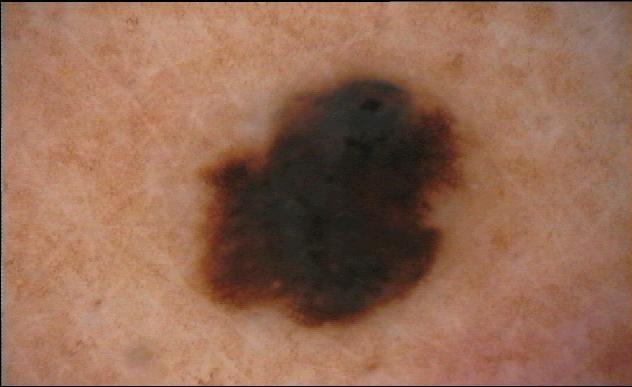
\includegraphics[width = 0.27\textwidth]{Chapter3/Figures/D540.jpg}}
\subfloat[\ac{rdgm}]{ 
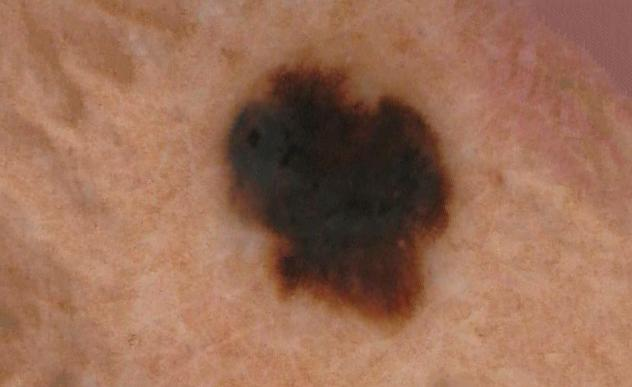
\includegraphics[width = 0.27\textwidth]{Chapter3/Figures/D540-deform1.jpg}}
\subfloat[\ac{bd}]{
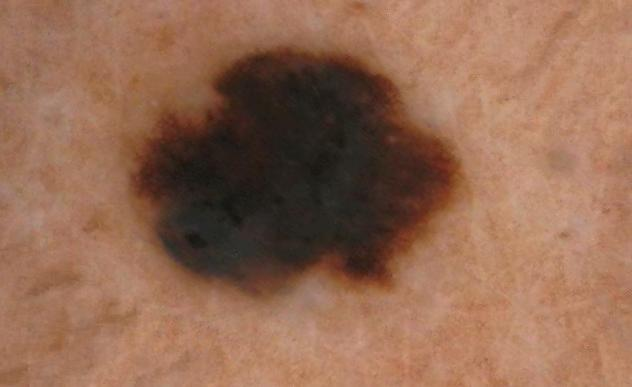
\includegraphics[width = 0.27\textwidth]{Chapter3/Figures/D540-deform2.jpg}}
\caption[Data space over sampling example]{Example of a melanoma lesion from Vienna dataset and its deformed generated samples. (a) \ac{rdgm}, (b) \ac{bd}.}
\label{fig:DSOS-example}
\end{figure}

Using this approach, based on 98 original melanoma lesions, 196 synthetic images were created.
From a total of 294 melanoma lesions (98$\times$3), 60$\%$ were kept for training, 20$\%$ for testing and another 20$\%$ for validation.
Therefore, to ensure balance training, the training set contained 174 melanoma lesions (58 original melanoma samples randomly selected from 98 lesions and their deformed images) and 174 dysplastic lesions randomly selected from 993 dysplastic nevi.
Besides 60 melanoma lesions (20 original samples and their 40 deformed samples), both the validation and test sets contained half of the remaining dysplastic lesions.
Table~\ref{tab:Exp2TTVlist} tabulates the number of melanoma and dysplastic lesions in each set.
\begin{table}[t]
\caption[A list of melanoma and dysplastic lesions in the \ac{dos}-balanced training, Experiment~\#2]{
	A list of melanoma and dysplastic lesions in the training, testing and validation sets of each subset. 
	10 different subsets were created by randomly selecting \#~lesions from the dataset. 
	If a melanoma lesion was selected to be a part of a specific group, its two deformed synthetic samples were also included in that set.}
\label{tab:Exp2TTVlist}
\medskip
\centering	
\footnotesize{
\begin{tabularx}{0.8\linewidth}{l	cccc}
\toprule
Set & \#~Melanoma & \#~$Melanoma_{D1}$ & \#~Melanoma$_{D2}$ & \#~Dysplastic\\
\midrule
Training & 58  & 58 & 58 & 174 \\
Test & 20 & 20 & 20 & 410 \\
Validation & 20 &  20 & 20 & 409 \\  
  \bottomrule
  \end{tabularx}
  }
\end{table}

Similar to our previous experiment, 10 different subsets were selected, while in each subset, the lesions were randomly selected for each of training, testing, and validation sets.
The validation set was only used with the \ac{svm} classifier.

In this experiment, only global mapping is used and the features are extracted from a window bounded to lesion boundaries.
All the lesions were segmented using a fusion approach rather than only a \ac{pdf}-based.
Individual and combinations of extracted features were further classified using \ac{rf} and RBF-\ac{svm} classifiers.
The results obtained are listed in Table.~\ref{tab:globalmapExp2}.
The best performance concerning individual and combined features are highlighted in bold.
%% Table 7
\begin{table}[t]
	\caption[Results of Experiment~\#2 - \ac{dos}-balance-training case]{The classification results after applying the \ac{dos} balancing method to the Vienna M~vs.~D subset.
	The data were classified using \ac{rf} and RBF-\ac{svm}.
	The results are indicated in terms of \acf{se} and \acf{sp} percentages.}
	\label{tab:globalmapExp2}
	\medskip
		
	\footnotesize{
%\resizebox{0.8\textwidth}{!}{
	\begin{center}
	\begin{tabularx}{0.73\textwidth}{@{}l	lllr	 ll	lllr	 @{}}
	\toprule
	Features & \multicolumn{4}{l}{\ac{rf}} & & & \multicolumn{4}{l}{\ac{svm}} \\
	\cmidrule{2-5} \cmidrule{8-11} 
	& \ac{se} & & & \ac{sp} & & &  \ac{se} & & & \ac{sp} \\
	\cmidrule{2-11}
	Individual Features\\
	\multicolumn{11}{l}{}\\[-1ex]
 $T_1$ & 72.00	& & & 77.97 & & &  69.00 & & & 68.63\\
 $T_2$ & 73.50	& & & 87.19 & & &  70.50	 & & & 89.32\\
 $T_3$ & \cellcolor[gray]{0.8}74.17	&\cellcolor[gray]{0.8} &\cellcolor[gray]{0.8} & \cellcolor[gray]{0.8}82.96	& & &  65.83	 & & & 74.65\\
 $T_4$ & \cellcolor[gray]{0.8}74.67	&\cellcolor[gray]{0.8} &\cellcolor[gray]{0.8} & \cellcolor[gray]{0.8}90.54    & & &  \cellcolor[gray]{0.8}78.00 &\cellcolor[gray]{0.8} &\cellcolor[gray]{0.8} & \cellcolor[gray]{0.8}78.78\\
 $C_1$ & \cellcolor[gray]{0.8}80.33	&\cellcolor[gray]{0.8} &\cellcolor[gray]{0.8} & \cellcolor[gray]{0.8}92.20	& & &  61.67	 & & & 74.40\\
 $C_2$ & \cellcolor[gray]{0.8}80.17	&\cellcolor[gray]{0.8} &\cellcolor[gray]{0.8} & \cellcolor[gray]{0.8}92.05	& & &  73.50	 & & & 76.60\\
  $S$  & 72.67	& & & 81.25	& & &  62.50	 & & & 69.10\\	
	\multicolumn{11}{l}{}\\
	Combined Features\\
	\multicolumn{11}{l}{}\\[-1ex]
$C_1,C_2	$					& \cellcolor[gray]{0.8}81.17 &\cellcolor[gray]{0.8} &\cellcolor[gray]{0.8} & \cellcolor[gray]{0.8}92.49 & & & 67.17 & & & 81.42\\
$C_1,C_2,S$					& 80.83	& & & 92.74	& & & 67.17 & & & 78.00\\
$T_1,T_2$ 					& 76.50	& & & 87.73	& & & 72.17 & & & 85.43\\
$T_1,T_3$					& 75.50	& & & 84.40	& & & 73.17	& & & 74.74\\
$T_1,T_4$					& 79.17	& & & 89.22	& & & 63.00	& & & 73.86\\
$T_1,T_2,T_3,T_4$			& 79.83	& & & 91.30	& & & 68.00	& & & 82.03\\
$T_1,T_2,C_1,C_2$			& \cellcolor[gray]{0.8}82.00	& \cellcolor[gray]{0.8}& \cellcolor[gray]{0.8}& \cellcolor[gray]{0.8}94.23	& & & 73.50	& & & 82.76\\
$T_1,T_3,C_1,C_2$			& \cellcolor[gray]{0.8}81.33	&\cellcolor[gray]{0.8} &\cellcolor[gray]{0.8} & \cellcolor[gray]{0.8}94.47	& & & 67.00	& & & 80.81\\
$T_1,T_3,T_4$				& 79.50	& & & 90.22	& & & 64.83	& & & 78.63\\
$T_1,C_1,C_2$				& \cellcolor[gray]{0.8}82.00 &\cellcolor[gray]{0.8} & \cellcolor[gray]{0.8}& \cellcolor[gray]{0.8}94.13 & & & 66.50	& & & 80.88\\
$T_3,C_1,C_2$				& 80.17	& & & 93.35	& & & 68.50	& & & 79.83\\
$T_4,C_1,C_2$				& 80.83	& & & 93.33	& & & 67.83	& & & 81.96\\
$T_1,T_2,C_1,C_2,S$			& \cellcolor[gray]{0.8}82.33 &\cellcolor[gray]{0.8} &\cellcolor[gray]{0.8} & \cellcolor[gray]{0.8}94.47	& & & 66.50	& & & 81.05\\
$T_1,T_2,T_3,T_4,C_1,C_2$	& \cellcolor[gray]{0.8}80.83	&\cellcolor[gray]{0.8} &\cellcolor[gray]{0.8} & \cellcolor[gray]{0.8}95.11	& & & 69.67	& & & 84.82\\
$T_1,T_2,T_3,C_1,C_2,S$		& \cellcolor[gray]{0.8}81.67	&\cellcolor[gray]{0.8} & \cellcolor[gray]{0.8}& \cellcolor[gray]{0.8}94.74	& & & 70.83	& & & 82.08\\
$T_1,T_2,T_3,T_4,C_1,C_2,S$  & 80.67	& & & 95.01	& & & 67.83	& & & 84.25\\	
 	\multicolumn{11}{l}{}\\
 	\bottomrule
  \end{tabularx}  
  \end{center}
	}
	
\end{table}
	



	




	


























	

















To be able to compare and evaluate the effects of having more melanoma samples in the balance training set, two different cases without using any balancing strategy, beside our inital proposed case with balancing strategy are considered:
(i) case~1: \ac{dos}-balance training, (ii) case~2: balance-training, and (iii) case~3: imbalance-training.
The second case considered balance training only using the original data.
Accordingly, in this case, our training set included 58 melanoma and 58 dysplastic, the test set had 20 melanoma and 468 dysplastic, and the validation set contained 20 melanona and 461 dysplastic.
Case~3 considered imbalance training, by removing the synthetic samples from each of the training, testing and validation sets.
For the sake of comparison of the three cases, only the results obtained by the best performing feature sets (i.e. the results highlighted in gray cell colors in Table~\ref{tab:globalmapExp2}) are listed in Table~\ref{tab:threecasecomExp2}.
%% Table 8
\begin{table}
	\caption[Results of Experiment~\#2 - comparison of the three cases]{Comparison of the classification results on the \ac{dos}-balanced, balanced, and imbalanced training cases.
	Each case was tested with the \ac{rf} and \ac{svm} classifiers. 
	The first part of the table shows the results obtained with \ac{rf}, while the second part lists the results achieved with \ac{svm}.
	The results are indicated in terms of the \acf{se} and \acf{sp} percentages.}
	\label{tab:threecasecomExp2}
	\medskip		
	\footnotesize{
%\resizebox{0.8\textwidth}{!}{
	\begin{center}
	\begin{tabularx}{0.95\textwidth}{@{}l	lllr	 ll	lllr	 ll lllr @{}}
	\toprule
	\multicolumn{17}{c}{ \ac{rf} classifier}\\
	\midrule
	Features & \multicolumn{4}{l}{\ac{dos}-balanced training} & & & \multicolumn{4}{l}{balanced training} & & & \multicolumn{4}{l}{imbalanced training} \\
	\cmidrule{2-5} \cmidrule{8-11} \cmidrule{14-17}
	& \ac{se} & & & \ac{sp} & & &  \ac{se} & & & \ac{sp} & & & \ac{se} & & & \ac{sp} \\
	\cmidrule{2-17}
	Individual Features\\
	\multicolumn{11}{l}{}\\[-2ex]
 $T_3$ & \cellcolor[gray]{0.8}74.17	&\cellcolor[gray]{0.8} &\cellcolor[gray]{0.8} & \cellcolor[gray]{0.8}82.96	 & & & 63.50	 & & & 64.82 & & & 23.00	& & & 94.35 \\
 $T_4$ & \cellcolor[gray]{0.8}74.67	&\cellcolor[gray]{0.8} &\cellcolor[gray]{0.8} & \cellcolor[gray]{0.8}90.54 & & & 59.50	 & & & 62.48 & & & 20.00	& & & 93.64 \\
 $C_1$ & \cellcolor[gray]{0.8}80.33	&\cellcolor[gray]{0.8} &\cellcolor[gray]{0.8} & \cellcolor[gray]{0.8}92.20 & & & 74.00 & & & 71.39 & & & 39.50 & & & 92.96 \\
 $C_2$ & \cellcolor[gray]{0.8}80.17	&\cellcolor[gray]{0.8} &\cellcolor[gray]{0.8} & \cellcolor[gray]{0.8}92.05	 & & & 71.00 & & & 58.44 & & & 38.00 & & & 92.84 \\
 	\multicolumn{17}{l}{}\\
	Combined Features\\
	\multicolumn{17}{l}{}\\[-2ex]
$C_1,C_2	$					& \cellcolor[gray]{0.8}81.17 &\cellcolor[gray]{0.8} &\cellcolor[gray]{0.8} & \cellcolor[gray]{0.8}92.49 & & & 74.50 & & & 64.58 & & & 43.00	 & & & 93.72\\
$T_1,T_2,C_1,C_2$			& \cellcolor[gray]{0.8}82.00	&\cellcolor[gray]{0.8} &\cellcolor[gray]{0.8} & \cellcolor[gray]{0.8}94.23	& & & 73.50 & & & 72.91 & & & 46.50 & & & 95.06\\
$T_1,T_3,C_1,C_2$			& \cellcolor[gray]{0.8}81.33	&\cellcolor[gray]{0.8} &\cellcolor[gray]{0.8} & \cellcolor[gray]{0.8}94.47	& & & 76.00 & & & 73.28 & & & 44.00 & & & 95.57\\
$T_1,C_1,C_2$				& \cellcolor[gray]{0.8}82.00	&\cellcolor[gray]{0.8} &\cellcolor[gray]{0.8} & \cellcolor[gray]{0.8}94.13	& & & 76.00	& & & 72.78 & & & 44.50 & & & 95.21\\
$T_1,T_2,C_1,C_2,S$			& \cellcolor[gray]{0.8}82.33	&\cellcolor[gray]{0.8} &\cellcolor[gray]{0.8} & \cellcolor[gray]{0.8}94.47	& & & 75.50	 & & & 72.42& & & 43.50 & & & 95.33\\
$T_1,T_2,T_3,T_4,C_1,C_2$	& \cellcolor[gray]{0.8}80.83	&\cellcolor[gray]{0.8} &\cellcolor[gray]{0.8} & \cellcolor[gray]{0.8}95.11	& & & 75.00	& & & 72.59 & & & 43.00 & & & 95.84\\
$T_1,T_2,T_3,C_1,C_2,S$		& \cellcolor[gray]{0.8}81.67	&\cellcolor[gray]{0.8} &\cellcolor[gray]{0.8} & \cellcolor[gray]{0.8}94.74	& & & 74.50 & & & 72.96 & & & 44.00 & & & 95.45\\
 	\multicolumn{17}{l}{}\\
% 	\bottomrule
  \end{tabularx}  
  \bigskip
	\begin{tabularx}{0.95\textwidth}{@{}l	lllr	 ll	lllr	 ll lllr @{}}
	\toprule
	\multicolumn{17}{c}{ \ac{svm} classifier}\\
	\midrule
	Features & \multicolumn{4}{l}{\ac{dos}-balanced training} & & & \multicolumn{4}{l}{balanced training} & & & \multicolumn{4}{l}{imbalanced training} \\
	\cmidrule{2-5} \cmidrule{8-11} \cmidrule{14-17}
	& \ac{se} & & & \ac{sp} & & &  \ac{se} & & & \ac{sp} & & & \ac{se} & & & \ac{sp} \\
	\cmidrule{2-17}
	Individual Features\\
	\multicolumn{17}{l}{}\\[-2ex]
 $T_3$ & \cellcolor[gray]{0.8}65.83 &\cellcolor[gray]{0.8} &\cellcolor[gray]{0.8} & \cellcolor[gray]{0.8}74.65 & & & 71.00 & & & 58.89 & & & 4.50 & & & 99.00\\
 $T_4$ & \cellcolor[gray]{0.8}78.00 &\cellcolor[gray]{0.8} &\cellcolor[gray]{0.8} & \cellcolor[gray]{0.8}78.78 & & & 47.50 & & & 62.33 & & & 5.00 & & & 97.53 \\
 $C_1$ & \cellcolor[gray]{0.8}61.67 &\cellcolor[gray]{0.8} &\cellcolor[gray]{0.8} & \cellcolor[gray]{0.8}74.40 & & & 45.00 & & & 85.76 & & & 3.00	 & & & 99.49\\
 $C_2$ & \cellcolor[gray]{0.8}73.50 &\cellcolor[gray]{0.8} &\cellcolor[gray]{0.8} & \cellcolor[gray]{0.8}76.60 & & & 66.50 & & & 65.20 & & & 4.00 & & & 99.63\\
	\multicolumn{17}{l}{}\\
	Combined Features\\
	\multicolumn{17}{l}{}\\[-2ex]
$C_1,C_2	$					& \cellcolor[gray]{0.8}67.17 &\cellcolor[gray]{0.8} &\cellcolor[gray]{0.8} & \cellcolor[gray]{0.8}81.42 & & & 52.00 & & & 80.26 & & & 0.00 & & & 100.00 \\
$T_1,T_2,C_1,C_2$			& \cellcolor[gray]{0.8}73.50	&\cellcolor[gray]{0.8} &\cellcolor[gray]{0.8} & \cellcolor[gray]{0.8}82.76 & & & 56.50 & & & 78.29 & & & 0.00 & & & 100.00\\
$T_1,T_3,C_1,C_2$			& \cellcolor[gray]{0.8}67.00	&\cellcolor[gray]{0.8} &\cellcolor[gray]{0.8} & \cellcolor[gray]{0.8}80.81 & & & 65.50 & & & 74.99 & & & 0.00 & & & 99.98\\
$T_1,C_1,C_2$				& \cellcolor[gray]{0.8}66.50	&\cellcolor[gray]{0.8} &\cellcolor[gray]{0.8} & \cellcolor[gray]{0.8}80.88 & & & 68.50 & & & 76.60 & & & 0.50 & & & 99.95\\
$T_1,T_2,C_1,C_2,S$			& \cellcolor[gray]{0.8}66.50	&\cellcolor[gray]{0.8} &\cellcolor[gray]{0.8} & \cellcolor[gray]{0.8}81.05 & & & 56.00 & & & 81.48 & & & 0.00 & & & 100.00\\
$T_1,T_2,T_3,T_4,C_1,C_2$	& \cellcolor[gray]{0.8}69.67	&\cellcolor[gray]{0.8} &\cellcolor[gray]{0.8} & \cellcolor[gray]{0.8}84.82 & & & 63.50 & & & 75.87 & & & 13.00 & & & 97.33\\
$T_1,T_2,T_3,C_1,C_2,S$		& \cellcolor[gray]{0.8}70.83	&\cellcolor[gray]{0.8} &\cellcolor[gray]{0.8} & \cellcolor[gray]{0.8}82.08 & & & 63.00 & & & 76.70 & & & 6.00 & & & 98.73\\
 	\multicolumn{17}{l}{}\\
 	\bottomrule
  \end{tabularx}  
	
	
	
	
\end{center}
 }
\end{table}
	



	




	


























	

















The first part of this table shows the results obtained with the \ac{rf} classifier for the three cases and the second part shows the results obtained with the \ac{svm}.


\subsubsection{Discussion}
The results listed in Table~\ref{tab:threecasecomExp2} indicate the benefits of \ac{dos}-balancing and balanced training in general.
It is clear that imbalanced training, as expected, overfits the majority class. 
In this case, the performance of the \ac{svm} was poorer, but \ac{rf} was also biased towards the majority class.

In the balanced training case (without the \ac{dos} balancing), the \ac{rf} ensemble achieved a mean \ac{se} and \ac{sp} of 69$\%$ and 67$\%$, respectively. 
In turn, the \acs{svm} reached an average \ac{se} and \ac{sp} of 61$\%$ and 71$\%$, respectively. 
These results indicate that the classifiers performed slightly better than average, with many  \acf{fp} samples (approximately more than 100 dysplastic lesions were classified as melanoma in each test). 
In comparison, in the \ac{dos}-balanced training case, the average \ac{se} and \ac{sp} over all the features, were measured at 79$\%$ and 91$\%$, respectively.
The results show that besides increasing the \ac{se}, the amount of \ac{fp} predictions was reduced notably (25--37 dysplastic lesions were misclassified). 
In general, the performance of the \ac{rf} classifier was superior to the \ac{svm} in this experiment.

\subsubsection{Conclusion}
The tests carried out in this experiment highlight the importance of a balanced training and balancing strategies. 
Data space over-sampling method granted the possibility of a balanced training using more samples from the dataset without reducing the test set. 
Increasing the training set by a factor of 3 improved the results remarkably. 
And it may be expected that balanced training with more samples will lead to even better results.

%----------------------------------------------------------------------------------------------------------------------------------------------------
\subsection{Experiment~\#3\\
\small{Melanoma~.vs~ Benign and Dysplastic nevi, Ensemble approach on PH$^{2}$ dataset}}
This experiment was conducted to evaluate the impact of the ensembles and features selected in the experiments~\#1 and \#2 on the PH$^{2}$~\cite{mendoncca2013ph} dataset.
This dataset contains 40 melanoma, 80 benign and 80 dysplastic lesions with their respective groundtruth segmentations, so there was no need to apply our segmentation algorithm.
%The segmentation of all the lesions are provided as well, therefore we did not perform our implemented segmentation approach.
In this experiment, we used a subset of 193 images, which included 39 melanoma, 78 benign and 76 dysplastic lesions.
Seven images were excluded due to artifacts.

In Sect.~\ref{sec:chp3-sec2}, we mentioned the research studies that employed this dataset~\cite{barata2013two,barata2013towards,ruela2013role,ruela2013color}.
Among these, Barata~et al.\,\cite{barata2013two} was highlighted as the main benchmark for future comparison.
In this work, the authors used locally and globally mapped color and gradient features. 
The locally mapped features were represented by the \ac{bow} approach and were classified by means of \ac{adb}, the \ac{svm} and k-\ac{nn}.
The benchmark results reported in~\cite{barata2013two} are listed in Table~\ref{tab:PH2benchmark}.
Since the \ac{bow} representation was already explored by the authors, and also due to the fact that \ac{bow} did not outperform the \ac{rf} ensemble on global features in Experiment~\#1, we chose to test only the ensemble performance in this experiment.
\begin{table}[t]
\caption[The PH$^{2}$ benchmark results]{Benchmark results on the PH$^{2}$ dataset using locally and globally mapped color and texture features~\cite{barata2013two}. The results are given in terms of the \ac{se} and \ac{sp} percentages.}
\label{tab:PH2benchmark}
\medskip
\centering	
\footnotesize{
\begin{tabularx}{0.5\linewidth}{l cr ll cr}
\toprule
 & \multicolumn{6}{c}{Features}\\
 \cmidrule{2-7}
 & \multicolumn{2}{c}{Color} & & & \multicolumn{2}{c}{Gradients} \\
\cmidrule{2-3} \cmidrule{6-7}
 & Global & Local &  &  &  Global & Local \\
\midrule
\ac{se} & 90  &  93   & & &  93  &  88  \\
\ac{sp} & 89  &  84   & & &  78  &  76  \\
 
  \bottomrule
  \end{tabularx}
  }
\end{table}


Here, we used the same individual and combined features as in Experiment~\#1.
These features were globally mapped from the lesions' segmented areas and were represented in their original feature space.
\ac{rf} and weighted combination ensembles were used.
The \ac{rf} ensemble was trained with 100 unpruned trees, while the weighted ensemble was created based on the combination of the \ac{svm}, an \ac{lda}, and \ac{rf}.
We also employed performance weighting, which makes the weight of each base learner proportional to its sensitivity performance on the validation set. 
We chose sensitivity instead of accuracy, because in cancer classification, \ac{se} has more importance than \ac{acc}.

The framework in this experiment was evaluated using \ac{loocv} in line with the PH$^{2}$ benchmark~\cite{barata2013two}.
In order to tackle the class imbalance problem, Barata.~et al\,\cite{barata2013two} suggested replicating melanoma features in the training set using additional Gaussian noise ($N(\mu, \sigma) = N(0, 0.0001)$).
Our approach, similar to Experiment~\#2, was to use the data space and generate synthetic melanoma images by deforming the originals using the \ac{bd} and \ac{rdgm} methods.
This technique yielded a nearly balanced dataset with 117 melanoma and 154 benign and dysplastic lesions.
During the evaluation, if a melanoma sample was included in a test set, its two synthetic images were included as well.
Besides, there was no need for the validation set for \ac{rf}, but half of the training set was kept for the validation of the weighted combination ensemble.
%Since \ac{rf} is created based on the bootstraps of the training set, there was no need for the validation set, in the contrary to weighted combination ensemble where half of the training set was kept for the validation set.
The results of this experiment are presented in Table~\ref{tab:globalmapExp3}.

%% Table 9
\begin{table}[t]
	\caption[Results of Experiment~\#3]{Classification results of the \ac{rf} and weighted combination (\ac{rf}, \ac{lda}, and \ac{svm}) ensemble approaches with the PH$^{2}$ dataset. %Two ensemble, \ac{rf} and weighted combination (\ac{rf}, \ac{lda}, and \ac{svm}) are used.
	The results are presented in terms of the \ac{se} and \ac{sp} percentages.}
	\label{tab:globalmapExp3}
	\medskip
		
	\footnotesize{
%\resizebox{0.8\textwidth}{!}{
	\begin{center}
	\begin{tabularx}{0.74\textwidth}{@{}l	lllr	 ll	lllr	 @{}}
	\toprule
	Features & \multicolumn{4}{l}{\ac{rf}} & & & \multicolumn{4}{l}{$\{$\ac{svm},\ac{lda},\ac{rf}$\}$} \\
	\cmidrule{2-5} \cmidrule{8-11} 
	& \ac{se} & & & \ac{sp} & & &  \ac{se} & & & \ac{sp} \\
	\cmidrule{2-11}
	Individual Features\\
	\multicolumn{11}{l}{}\\[-1ex]
 $T_1$ & 62.39	& & & 82.47 & & &  54.78 & & & 75.97\\
 $T_2$ & 72.65	& & & 88.39 & & &  64.10	 & & & 82.47\\
 $T_3$ & 82.05	& & & 85.71	& & &  63.38	 & & & 77.92\\
 $T_4$ & 88.03	& & & 90.91 & & &  62.07	 & & & 85.71\\
 $C_1$ & 88.89	& & & 94.16 	& & &  59.83	 & & & 93.51\\
 $C_2$ & 89.74	& & & 90.91	& & &  75.21	 & & & 90.26\\
  $S$  & 76.92	& & & 90.26	& & &  62.39	 & & & 86.36\\	
	\multicolumn{11}{l}{}\\
	Combined Features\\
	\multicolumn{11}{l}{}\\[-1ex]
$C_1,C_2	$					& \cellcolor[gray]{0.8}93.16 &\cellcolor[gray]{0.8} &\cellcolor[gray]{0.8} & \cellcolor[gray]{0.8}94.16 & & & 76.07 & & & 94.16\\
$C_1,C_2,S$					& 90.06 	& & & 94.81	& & & 81.74 & & & 92.21\\
$T_1,C_2$					& \cellcolor[gray]{0.8}94.02	&\cellcolor[gray]{0.8} &\cellcolor[gray]{0.8} & \cellcolor[gray]{0.8}92.21	& & & 70.94	& & & 90.91\\
$T_1,C_1,C_2$				& \cellcolor[gray]{0.8}93.16	&\cellcolor[gray]{0.8} &\cellcolor[gray]{0.8} & \cellcolor[gray]{0.8}93.51	& & & 75.21	& & & 94.81\\
$T_3,C_1,C_2$				& 89.74 & & & 95.45	& & & 86.32	& & & 94.81\\
$T_4,C_1,C_2$				& 89.74 & & & 92.86	& & & 88.03	& & & 92.21\\
$T_1,T_2,T_3,T_4$			& 90.06	& & & 92.21	& & & 86.32	& & & 92.16\\
$T_1,T_3,C_1,C_2$			& \cellcolor[gray]{0.8}92.31	&\cellcolor[gray]{0.8} &\cellcolor[gray]{0.8} & \cellcolor[gray]{0.8}93.51	& & & 67.54	& & & 93.51\\
$T_1,T_2,T_3,T_4,C_1,C_2$	& 91.45	& & & 94.16	& & & 89.74	& & & 93.51\\
$T_1,T_2,T_3,T_4,C_1,C_2 $  & 91.45	& & & 94.16	& & & \cellcolor[gray]{0.8}92.31 &\cellcolor[gray]{0.8} &\cellcolor[gray]{0.8} & \cellcolor[gray]{0.8}92.86\\
$T_1,T_2,T_3,T_4,C_1,C_2,S$ & 91.45	& & & 93.51	& & & 88.89	& & & 94.16\\	
 	\multicolumn{11}{l}{}\\
 	\bottomrule
  \end{tabularx}  
  \end{center}
	}
	
\end{table}
	



	




	


























	


















\subsubsection{Discussion}
The comparison between the current experiment's results and the benchmark reveals the potential of the proposed method. 
In Table~\ref{tab:globalmapExp3}, the figures showing a better outcome than the benchmark are highlighted in bold. 
The highest performance of the benchmark, as shown in Table~\ref{tab:PH2benchmark}, was achieved by the \ac{bow} representation of locally mapped color features with \ac{se} and \ac{sp} of 93$\%$ and 84$\%$, respectively.
The global mapping of the gradient features showed the second best \ac{se} and \ac{sp} of 93$\%$ and 78$\%$, respectively.
In this experiment, the combination of colors ($C_{1},C_{2}$), \ac{clbp} and opponent color angle ($T_{1},C_{2}$), and the \ac{clbp} and both color features ($T_{1},C_{1},C_{2}$) outperformed the benchmark.
Among these, ($T_{1},C_{2}$) achieved the best \ac{se} and \ac{sp} of 94.02$\%$ and 92.21$\%$, respectively.
As for the ensemble performance, \ac{rf} proved better than the weighted combination of \ac{rf}, the \ac{lda} and the \ac{svm}. 
This could be due to the fact that with a validation set, the base learners of the weighted combination ensemble are trained on half of the training data, which may have weakened its performance.

\subsubsection{Conclusion}
We proposed an automated classification framework based on a global feature extraction and ensemble learning. 
The framework was designed for the differentiation of melanoma from benign and dysplastic lesions.
The evaluation results from the PH$^{2}$ dataset demonstrated that ensembles such as \ac{rf} outperform single learner methods.
Using the \ac{rf} ensemble on globally mapped color and texture features, our framework achieved the highest \ac{se} and \ac{sp} of 94$\%$ and 92$\%$, respectively.
In general, the results confirm the role and importance of color features for the detection and discrimination of melanoma lesions.
However, the significance of texture features omitted in previous research works cannot be denied. 

%--------------------------------------------------------------------------------------------------------------------------------------------------
\subsection{Experiment~\#4\\
\small{Melanoma~vs.~Benign and Dysplastic nevi, Study of balancing techniques on $PH^{2}$ dataset}}
\label{subsec:chp3-exp4}
This experiment studies the effect of balancing strategies on melanoma classification.
In order to make future comparisons possible, we chose to work with the PH$^{2}$ dataset. 
The experiment was conducted on a subset of the original dataset with an imbalance ratio of 1:3, which was chosen deliberately to comply with the requirements of the \ac{dos} method.
The \ac{dos} method synthetically generates two additional melanoma images by deforming the original sample. 
Subsequently, the subset was composed of 39 melanoma and 117 benign and dysplastic lesions, which were randomly selected.

Based on the results of Experiment~\#3, we considered two color features (color statistics ($C_{1}$) and the opponent color angle space ($C_{2}$)) and two texture features (\ac{clbp} ($T_{1}$) and  Gabor filters ($T_{3}$)).
Using these individual features and their combinations, the 9 following feature sets were compared; $\{ C_{1}; C_{2}; C_{1,2}; T_{1}; T_{3}; T_{1,3}; \{T_{1}, C_{1,2}\}; \{T_{2}, C_{1,2}\}; \{T_{1,2}, C_{1,2}\}\}$.
These features were globally extracted from the segmented part of each sample and were represented in their original space.
Twelve different balancing techniques, \ac{dos}, \ac{ros}, \ac{smote}, \ac{rus}, \ac{tl}, \ac{cus}, \ac{nm1}, \ac{nm2}, \ac{nm3}, \ac{ncr}, \ac{smote}+\ac{enn}, and \ac{smote}+\ac{tl}, were used to create a balanced training set.
We used the \ac{rf} classifier with 100 unpruned trees and the original feature dimension of size $M = \{144, 84, 228, 26, 48, 74, 254, 276, 302\}$.

In order to validate the classifier with a stratified sampling, we used a 10-fold cross-validation scheme.
However, contrary to the common 10-fold cross-validation, at each iteration, eight folds were kept for training and two for testing. 
%The training set is balance using previously described imbalance techniques (see Sect.~\ref{sec:chp2-sec5}). 
%The classification performance is reported in terms of the average \ac{se}~(TPR) and \ac{sp}~(TNR) over the 10 cross-validation runs. 
In order to find the best performance, similar to \cite{barata2013towards}, we used a cost function, which provides a trade-off between the \ac{se} and \ac{sp}.
It is formulated as follows:

\begin{equation}\label{eq:cost}
C = \frac{c_{10}(1-\ac{se})+c_{01}(1-\ac{sp})}{c_{10}+c_{01}} \,,
\end{equation}

\noindent where $c_{10}$ and $c_{01}$ are the costs of incorrectly classifying melanoma and non-melanoma lesions, respectively.
As it is more important to correctly classify melanoma lesions (i.e., high \ac{se}), $c_{10}$ should be penalized more.
%Since in cancer classification such as melanoma, correctly identifying the cancer lesions has high importance (i.e., high \ac{se}). 
%Thus incorrect classification of melanoma is not desired and $c_{10}$ is a greater error and evidently more costly and should be penalized more. 
In order to achieve a high \ac{se} without significantly reducing the value of \ac{sp}, Barata~et al. proposed setting $c_{10} = 1.5 \times c_{01}$ and $c_{01} = 1$~\cite{barata2013towards}.  
We considered the same configuration for our cost function. 

The classification results obtained in this experiment are reported in Table~\ref{tab:globalmapExp4}, which can be divided into three main parts that show the results for imbalanced data (IB), balancing in the data space (\ac{dos}) and balancing in the feature space.
These strategies are separated by double horizontal lines.
The strategies applied in the feature space are subdivided into either \ac{os}, \ac{us} or a combination of \ac{os} followed by \ac{us} (see horizontal dashed line in Table~\ref{tab:globalmapExp4}).
In this table, based on the cost function defined above, the best results for each feature set are highlighted in the shaded cells.
Table~\ref{tab:table11} shows the cost values for each configuration. 
Strategies with low cost functions are synonymous with a better \ac{se} and \ac{sp} trade-off.
\afterpage{
\begin{landscape}

\begin{table}
\caption[Results of Experiment~\#4]{\small{Results obtained with different balancing techniques for color and texture features using the \acs*{rf} classifier. The first and second highest results for each feature set are highlighted in gray colors.}}
\label{tab:globalmapExp4}
\medskip
\centering
%\begin{tabularx}{0.8\linewidth}
%\resizebox{1.4\textwidth}{!}{
\scriptsize{
\begin{tabularx}{1.15\textwidth}{@{}l cccccc		cccccc @{}}
\toprule
Features &  \multicolumn{6}{l}{Color}& \multicolumn{6}{l}{Texture} \\%& \multicolumn{6}{l}{Combined}\\
  \cmidrule(r){2-7}  \cmidrule(r){8-13}  %\cmidrule(r){14-19}  
		   & \multicolumn{2}{c}{$C_{1}$}& \multicolumn{2}{c}{$C_{2}$}& \multicolumn{2}{c}{$C_{1,2}$}& \multicolumn{2}{c}{$T_{1}$} &  \multicolumn{2}{c}{$T_{3}$} & \multicolumn{2}{c}{$T_{1,3}$}\\ %& \multicolumn{2}{c}{$T_{1},C_{1,2}$}& \multicolumn{2}{c}{$T_{2},C_{1,2}$}& \multicolumn{2}{c}{$T_{1,2},C_{1,2}$}\\ 
  \cmidrule(r){2-3}  \cmidrule(r){4-5} \cmidrule(r){6-7} \cmidrule(r){8-9} \cmidrule(r){10-11} \cmidrule(r){12-13} %\cmidrule(r){14-15} \cmidrule(r){16-17} \cmidrule(r){18-19} 
  Balancing techniques & \acs{se}& \acs{sp} & \acs{se} & \acs{sp} & \acs*{se} &\acs{sp} & \acs{se} & \acs{sp} & \acs{se} & \acs{sp} & \acs{se} & \acs{sp} \\ \midrule % & \acs{se} & \acs{sp} & \acs{se} & \acs{sp} & \acs{se} & \acs{sp}  \\ \midrule
\multicolumn{13}{l}{}\\[-2.3ex]
\multicolumn{1}{c}{IB} & 52.50 & 89.58 & 75.00 & 88.75 & 71.25& 87.50& 38.75 & 91.67 & 60.00 & 96.25 & 66.25 & 93.75 \\%&73.75 & 89.58&71.25 & 89.58 & 71.25& 92.50\\
\multicolumn{13}{l}{}\\[-2.3ex]
\midrule \midrule
\multicolumn{13}{l}{}\\[-2.3ex]
\multicolumn{1}{c}{\acs{dos}} &\cellcolor[gray]{0.8}93.75 &\cellcolor[gray]{0.8}66.67 &80.00 & 86.25& 82.50 & 87.08  & 43.75 &83.75 &\cellcolor[gray]{0.8}72.50&\cellcolor[gray]{0.8}90.00 & 70.00& 91.67 \\ % &77.50 & 87.08 &81.25 &88.33 &78.75 &88.33  \\
\multicolumn{13}{l}{}\\[-2.3ex]
\midrule \midrule
\multicolumn{13}{l}{}\\[-2.3ex]
\multicolumn{1}{c}{\acs{ros}} &55.00 & 80.83& 80.00 & 84.17& 72.50 &85.42 &42.50 & 82.08 &60.00 & 89.17 &66.25 &87.92 \\ %&75.00&85.42&73.75&86.25&73.75 &85.83\\
\multicolumn{13}{l}{}\\[-2.2ex]
\multicolumn{1}{c}{\acs{smote}} & 60.00 & 82.50 & 78.75 & 84.58 & 75.00 & 70.00 & 56.25 & 74.17 & 61.25 & 87.50 & 84.17 &87.08 \\ %& 78.75& 85.00 &73.75 & 84.58 &73.75&85.00 \\
\multicolumn{13}{l}{}\\[-2.3ex] 
\hdashline \noalign{\vskip 3pt}
\multicolumn{13}{l}{}\\[-2.3ex]
\multicolumn{1}{c}{\acs{rus}} & 72.50 & 72.92 & 86.25 & 80.00 & 78.75 &80.00 & 67.50 & 53.33 &76.25 &76.25  & 85.00 &78.75\\ % &91.25 &75.00 & 85.00 & 78.75 &92.50 &78.33\\
\multicolumn{13}{l}{}\\[-2.3ex]
\multicolumn{1}{c}{\acs{tl}} & 51.25 & 86.25 & 76.25 & 87.92&67.50 & 88.33  & 37.50 & 87.92 & 65.00 &90.42 & 68.75 & 91.67\\ % & 73.75 & 88.75 &63.75 & 90.00 & 72.50 & 91.25\\
\multicolumn{13}{l}{}\\[-2.3ex]
\multicolumn{1}{c}{\acs{cus}} & 81.25 & 67.92 & 80.00 & 84.58& 86.25 & 80.42 & 56.25 & 65.83 & 70.00 & 77.50 & 85.00 & 77.08\\% & 83.75 & 81.25 & 80.00 & 84.17 & 83.75 & 82.92\\
\multicolumn{13}{l}{}\\[-2.3ex]
\multicolumn{1}{c}{\acs{nm1}} & 67.50 & 72.08 & 86.25 & 79.17& 85.00 & 82.50 & 72.50 & 43.75 & 80.00 & 62.50 & 87.50 & 66.67\\ % & 85.00 & 82.08 & 86.25 &80.42 & 87.50 & 80.83\\
\multicolumn{13}{l}{}\\[-2.3ex]
\multicolumn{1}{c}{\acs{nm2}} & 70.00 & 72.92 & 86.25 & 81.25 & 85.00 & 82.92 & 76.25 & 48.75 & 86.25 & 40.83 & 86.25 & 51.25\\ %& \cellcolor[gray]{0.8}87.50 & \cellcolor[gray]{0.8}82.08 &\cellcolor[gray]{0.8}92.50 &\cellcolor[gray]{0.8}77.50&\cellcolor[gray]{0.8}91.25 &\cellcolor[gray]{0.8}81.67\\
\multicolumn{13}{l}{}\\[-2.3ex]
\multicolumn{1}{c}{\acs{nm3}} & 82.50 & 75.00 & 87.50 & 80.83 & 85.00 & 80.42 &73.75 & 55.83 & 72.50 & 82.50 & 82.50 & 80.42 \\ %& 83.75 & 81.25 & 85.00 & 80.00 & 86.25 & 80.42\\
\multicolumn{13}{l}{}\\[-2.3ex]
\multicolumn{1}{c}{\acs{ncr}} & 66.25 & 76.67 & \cellcolor[gray]{0.8} 87.50 &\cellcolor[gray]{0.8}81.25 & 85.00 & 82.08 & 67.50 & 67.92 & 75.00 & 85.83 & \cellcolor[gray]{0.8}82.50 & \cellcolor[gray]{0.8}83.33\\ % &  86.25 &  81.67 & 82.50  & 85.00 & 83.75  & 85.42\\
\multicolumn{13}{l}{}\\[-2.3ex]
\hdashline \noalign{\vskip 3pt}
\multicolumn{13}{l}{}\\[-2.3ex]
\multicolumn{1}{c}{\acs{smote} + \acs{enn}} & 76.25 & 73.33 & 85.00 & 81.25 & 85.00 & 82.08 &\cellcolor[gray]{0.8} 81.25 &\cellcolor[gray]{0.8} 56.25 & 76.25 & 82.08 & 80.00 & 79.58\\ % & 86.25 & 81.25 & 83.75 & 82.50 & 78.75 & 82.92\\
\multicolumn{13}{l}{}\\[-2.3ex]
\multicolumn{1}{c}{\acs{smote} + \acs{tl}} & 75.00 & 73.75 & 83.75 & 82.50 & \cellcolor[gray]{0.8}87.50 &\cellcolor[gray]{0.8}80.83 & 72.50 & 59.17 & 77.50 & 82.08 & 78.75 & 78.75\\ [-2.2ex]% & 85.00 & 82.08 & 77.50 & 82.92 & 88.75 & 82.50\\
%\multicolumn{13}{l}{}\\[-2.2ex]

\end{tabularx}

\bigskip

\begin{tabularx}{1.15\textwidth}{@{}l cccccc cccccc cccccccccc @{}}
\toprule
Features &  &  &  &  &  &  &  \multicolumn{6}{l}{Combined} &  &  &  &  &  &  &  &  &   \\
  \cmidrule(r){8-13}    
		 &  &  &  &  &  &  &  \multicolumn{2}{c}{$T_{1},C_{1,2}$}& \multicolumn{2}{c}{$T_{3},C_{1,2}$}& \multicolumn{2}{c}{$T_{1,3},C_{1,2}$} &  &  &  &  &  & &  &  & &\\ 
  \cmidrule(r){8-9}  \cmidrule(r){10-11} \cmidrule(r){12-13} 
  Balancing techniques &  &  &  &  &  &  & \acs{se}& \acs{sp} & \acs{se} & \acs{sp} & \acs{se} &\acs{sp} &  &  &  &  &  &  &  &  &  \\ 
\midrule 
%\cmidrule(r){1-2} \cmidrule(r){5-10}
\multicolumn{23}{l}{}\\[-2.3ex]
\multicolumn{1}{c}{IB} &  &  &  &  &  &  & 73.75 & 89.58 & 71.25 & 89.58 & 71.25 & 92.50 &  &  &  &  &  &  &  &  &  \\
\multicolumn{23}{l}{}\\[-2.3ex]
\midrule \midrule
\multicolumn{23}{l}{}\\[-2.3ex]
%\cmidrule(r){1-2} \cmidrule(r){5-10}
\multicolumn{1}{c}{\acs{os}} &  &  &  &  &  &  &  77.50 & 87.08 & 81.25 & 88.33 & 78.75 & 88.33 &  &  &  &  &  &  &  &  &  \\
\multicolumn{23}{l}{}\\[-2.3ex]
\midrule \midrule
\multicolumn{23}{l}{}\\[-2.3ex]
%\cmidrule(r){1} \cmidrule(r){5-10} 
\multicolumn{1}{c}{\acs{ros}} &  &  &  &  &  &  & 75.00 & 85.42 & 73.75 & 86.25 & 73.75 & 85.83 &  &  &  &  &  & &  &  &  \\
\multicolumn{23}{l}{}\\[-2.3ex]
\multicolumn{1}{c}{\acs{smote}} &  &  &  &  &  &  & 78.75 & 85.00 & 73.75 & 84.58 & 73.75 & 85.00 &  &  &  &  &  &  &  &  &  \\ 
\multicolumn{23}{l}{}\\[-2.3ex]
\hdashline \noalign{\vskip 3pt}
\multicolumn{23}{l}{}\\[-2.3ex]
%\chdashline{1-16}
\multicolumn{1}{c}{\acs{rus}} &  &  &  &  &  &  & 91.25 & 75.00 & 85.00 & 78.75 & 92.50 & 78.33 &  &  &  &  &  & &  &  &  \\
\multicolumn{23}{l}{}\\[-2.3ex]
\multicolumn{1}{c}{\acs{tl}}  &  &  &  &  &  &  & 73.75 & 88.75 & 63.75 & 90.00 & 72.50 & 91.25 &  &  &  &  &  & &  &  &  \\
\multicolumn{23}{l}{}\\[-2.3ex]
\multicolumn{1}{c}{\acs{cus}} &  &  &  &  &  &  & 83.75 & 81.25 & 80.00 & 84.17 & 83.75 & 82.92 &  &  &  &  &  & &  &  &  \\
\multicolumn{23}{l}{}\\[-2.3ex]
\multicolumn{1}{c}{\acs{nm1}} &  &  &  &  &  &  & 85.00 & 82.08 & 86.25 & 80.42 & 87.50 & 80.83 &  &  &  &  &  & &  &  & \\
\multicolumn{23}{l}{}\\[-2.3ex]
\multicolumn{1}{c}{\acs{nm2}} &  &  &  &  &  &  & \cellcolor[gray]{0.8}87.50 & \cellcolor[gray]{0.8}82.08 &\cellcolor[gray]{0.8}92.50 & \cellcolor[gray]{0.8}77.50 & \cellcolor[gray]{0.8}91.25 & \cellcolor[gray]{0.8}81.67 &  &  &  &  &  & &  &  &  &\\
\multicolumn{23}{l}{}\\[-2.3ex]
\multicolumn{1}{c}{\acs{nm3}} &  &  &  &  &  &  & 83.75 & 81.25 & 85.00 & 80.00 & 86.25 & 80.42 &  &  &  &  &  & &  &  &  \\
\multicolumn{23}{l}{}\\[-2.3ex]
\multicolumn{1}{c}{\acs{ncr}} &  &  &  &  &  &  & 86.25 & 81.67 & 82.50 & 85.00 & 83.75 & 85.42 &  &  &  &  &  & &  &  &  \\
\multicolumn{23}{l}{}\\[-2.3ex]
\hdashline\noalign{\vskip 3pt}
\multicolumn{23}{l}{}\\[-2.3ex]
\multicolumn{1}{c}{\acs{smote} + \acs{enn}} &  &  &  &  &  &  & 86.25 & 81.25 & 83.75 & 82.50 & 78.75 & 82.92 &  &  &  &  &  & &  &  &   \\
\multicolumn{23}{l}{}\\[-2.3ex]
\multicolumn{1}{c}{\acs{smote} + \acs{tl}}  &  &  &  &  &  &  & 85.00 & 82.08 & 77.50 & 82.92 & 88.75 & 82.50 &  &  &  &  &  & &  &  &  \\
\multicolumn{23}{l}{}\\[-2.3ex]
\bottomrule
\end{tabularx}
}

\end{table}

\normalsize \vfill
\end{landscape}

\begin{table}
\caption[Classification costs in Experiment~\#4]{The classification cost, $C$, for different balancing techniques and feature sets.}
\label{tab:table11}
\medskip
\centering

\footnotesize{
\resizebox{1\textwidth}{!}{
\begin{tabularx}{1.05\linewidth}{@{}l ccc ccc ccc @{}}

\toprule 
 Balancing techniques & \multicolumn{9}{c}{Classification cost, $C$} \\
 \cmidrule{2-10}
		   & $C_{1}$ & $C_{2}$ &  $C_{1,2}$ &  $T_{1}$  &  $T_{3}$  & $T_{1,3}$ &  $T_{1},C_{1,2}$ &  $T_{3},C_{1,2}$ &  $T_{1,3},C_{1,2}$ \\ 
  \midrule 
\multicolumn{10}{l}{}\\[-2.2ex]  
IB & 0.3267 &  0.1950 & 0.2225 & 0.4008 & 0.2550   & 0.2275 & 0.1992 & 0.2142 & 0.2025\\
\multicolumn{10}{l}{}\\[-2.2ex]
\midrule \midrule
\multicolumn{10}{l}{}\\[-2.2ex]
\ac{dos}&   				\cellcolor[gray]{0.8}0.1708 &  0.1750    		& 0.1567    		& 0.4025    			&\cellcolor[gray]{0.8}0.2050   & 0.2133 			& 0.1867  	
	  & 0.1592 			& 0.1742\\
\multicolumn{10}{l}{}\\[-2.2ex]
\midrule \midrule
\multicolumn{10}{l}{}\\[-2.2ex]
\ac{os}&					0.3467 			&  0.1833 			& 0.2233  		& 0.4167 			& 0.2833   & 0.2508 			& 0.2083 		  & 0.2125 			& 0.2142\\
\multicolumn{10}{l}{}\\[-2.2ex]
\ac{smote}&				0.3100  			&  0.1892  			& 0.2133   		& 0.3658   			& 0.2825   & 0.2317  		& 0.1875 		  & 0.2192 			& 0.2175\\
\multicolumn{10}{l}{}\\[-2.2ex]
\hdashline \noalign{\vskip 3pt}
\multicolumn{10}{l}{}\\[-2.2ex]
\ac{rus}&				0.2733 			&  0.1625   			& 0.2075   		& 0.3817   			& 0.2375   & 0.1750  		& 0.1525  		  & 0.1750 			& 0.1317\\
\multicolumn{10}{l}{}\\[-2.2ex]
\ac{tl}&					0.3475  			&  0.1908   			& 0.2417   		& 0.4233   			& 0.2483   & 0.2208  		& 0.2025  		  & 0.2575 			& 0.2000\\
\multicolumn{10}{l}{}\\[-2.2ex]
\ac{cus}&				0.2408  			&  0.1817   			& 0.1608   		& 0.3992   			& 0.2700   & 0.1817  		& 0.1725  		  & 0.1833 			& 0.1658\\
\multicolumn{10}{l}{}\\[-2.2ex]
\ac{nm1}& 				0.3067  			&  0.1658   			& 0.1600   		& 0.3900   			& 0.2700   & 0.2083  		& 0.1617   		  & 0.1608 			& 0.1517\\
\multicolumn{10}{l}{}\\[-2.2ex]
\ac{nm2}& 				0.2883  			&  0.1575   			& 0.1583   		& 0.3475   			& 0.3192   & 0.2775  		& \cellcolor[gray]{0.8}0.1467 &\cellcolor[gray]{0.8}0.1350  &\cellcolor[gray]{0.8}0.1258\\
\multicolumn{10}{l}{}\\[-2.2ex]
\ac{nm3}& 				0.2050  			&  0.1517   			& 0.1683   		& 0.3342   			& 0.2350   & 0.1833  		& 0.1725  		  & 0.1700  			& 0.1608\\
\multicolumn{10}{l}{}\\[-2.2ex]
\ac{ncr}& 				0.2958  			& \cellcolor[gray]{0.8}0.1500  & 0.1617   		& 0.3233   			& 0.2067   &\cellcolor[gray]{0.8}0.1717  & 0.1558  		  & 0.1650  			& 0.1558\\
\multicolumn{10}{l}{}\\[-2.2ex]
\hdashline \noalign{\vskip 3pt}
\multicolumn{10}{l}{}\\[-2.2ex]
\ac{smote}+\acs*{enn}& 	0.2492  			&  0.1650   			& 0.1617   		&\cellcolor[gray]{0.8}0.2875    & 0.2142   & 0.2017  		& 0.1575  		  & 0.1675  			& 0.1958\\
\multicolumn{10}{l}{}\\[-2.2ex]
\ac{smote}+\ac{tl}& 		0.2550 			&  0.1675   			&\cellcolor[gray]{0.8}0.1517 & 0.3283   		    & 0.2067   & 0.2125  		& 0.1617  		  & 0.2033  			& 0.1375\\
\multicolumn{10}{l}{}\\[-2.2ex]
\bottomrule

\end{tabularx}
}}
\end{table}

}
\subsubsection{Discussion}
The results of this experiment indicate that balancing techniques are essential for improving the classification performance. 
% Certainly, some techniques are more subjects to the feature representations than others. 
%However, the improvements in comparison to imbalanced classification is evident. 
Thus, the \ac{us} techniques and their combination with \ac{os} performed better than the \ac{os} techniques alone. 
In turn, the \ac{os} techniques applied in the data space outperformed those applied in the feature space.
Due to the similar characteristics of melanoma and dysplastic lesions, their images are expected to have overlapping feature spaces. 
Subsequently, the misleading samples could be removed using \ac{us} and thus ensure a better performance.
%\begin{landscape}

\begin{table}
\caption[Results of Experiment~\#4]{\small{Results obtained with different balancing techniques for color and texture features using the \acs*{rf} classifier. The first and second highest results for each feature set are highlighted in gray colors.}}
\label{tab:globalmapExp4}
\medskip
\centering
%\begin{tabularx}{0.8\linewidth}
%\resizebox{1.4\textwidth}{!}{
\scriptsize{
\begin{tabularx}{1.15\textwidth}{@{}l cccccc		cccccc @{}}
\toprule
Features &  \multicolumn{6}{l}{Color}& \multicolumn{6}{l}{Texture} \\%& \multicolumn{6}{l}{Combined}\\
  \cmidrule(r){2-7}  \cmidrule(r){8-13}  %\cmidrule(r){14-19}  
		   & \multicolumn{2}{c}{$C_{1}$}& \multicolumn{2}{c}{$C_{2}$}& \multicolumn{2}{c}{$C_{1,2}$}& \multicolumn{2}{c}{$T_{1}$} &  \multicolumn{2}{c}{$T_{3}$} & \multicolumn{2}{c}{$T_{1,3}$}\\ %& \multicolumn{2}{c}{$T_{1},C_{1,2}$}& \multicolumn{2}{c}{$T_{2},C_{1,2}$}& \multicolumn{2}{c}{$T_{1,2},C_{1,2}$}\\ 
  \cmidrule(r){2-3}  \cmidrule(r){4-5} \cmidrule(r){6-7} \cmidrule(r){8-9} \cmidrule(r){10-11} \cmidrule(r){12-13} %\cmidrule(r){14-15} \cmidrule(r){16-17} \cmidrule(r){18-19} 
  Balancing techniques & \acs{se}& \acs{sp} & \acs{se} & \acs{sp} & \acs*{se} &\acs{sp} & \acs{se} & \acs{sp} & \acs{se} & \acs{sp} & \acs{se} & \acs{sp} \\ \midrule % & \acs{se} & \acs{sp} & \acs{se} & \acs{sp} & \acs{se} & \acs{sp}  \\ \midrule
\multicolumn{13}{l}{}\\[-2.3ex]
\multicolumn{1}{c}{IB} & 52.50 & 89.58 & 75.00 & 88.75 & 71.25& 87.50& 38.75 & 91.67 & 60.00 & 96.25 & 66.25 & 93.75 \\%&73.75 & 89.58&71.25 & 89.58 & 71.25& 92.50\\
\multicolumn{13}{l}{}\\[-2.3ex]
\midrule \midrule
\multicolumn{13}{l}{}\\[-2.3ex]
\multicolumn{1}{c}{\acs{dos}} &\cellcolor[gray]{0.8}93.75 &\cellcolor[gray]{0.8}66.67 &80.00 & 86.25& 82.50 & 87.08  & 43.75 &83.75 &\cellcolor[gray]{0.8}72.50&\cellcolor[gray]{0.8}90.00 & 70.00& 91.67 \\ % &77.50 & 87.08 &81.25 &88.33 &78.75 &88.33  \\
\multicolumn{13}{l}{}\\[-2.3ex]
\midrule \midrule
\multicolumn{13}{l}{}\\[-2.3ex]
\multicolumn{1}{c}{\acs{ros}} &55.00 & 80.83& 80.00 & 84.17& 72.50 &85.42 &42.50 & 82.08 &60.00 & 89.17 &66.25 &87.92 \\ %&75.00&85.42&73.75&86.25&73.75 &85.83\\
\multicolumn{13}{l}{}\\[-2.2ex]
\multicolumn{1}{c}{\acs{smote}} & 60.00 & 82.50 & 78.75 & 84.58 & 75.00 & 70.00 & 56.25 & 74.17 & 61.25 & 87.50 & 84.17 &87.08 \\ %& 78.75& 85.00 &73.75 & 84.58 &73.75&85.00 \\
\multicolumn{13}{l}{}\\[-2.3ex] 
\hdashline \noalign{\vskip 3pt}
\multicolumn{13}{l}{}\\[-2.3ex]
\multicolumn{1}{c}{\acs{rus}} & 72.50 & 72.92 & 86.25 & 80.00 & 78.75 &80.00 & 67.50 & 53.33 &76.25 &76.25  & 85.00 &78.75\\ % &91.25 &75.00 & 85.00 & 78.75 &92.50 &78.33\\
\multicolumn{13}{l}{}\\[-2.3ex]
\multicolumn{1}{c}{\acs{tl}} & 51.25 & 86.25 & 76.25 & 87.92&67.50 & 88.33  & 37.50 & 87.92 & 65.00 &90.42 & 68.75 & 91.67\\ % & 73.75 & 88.75 &63.75 & 90.00 & 72.50 & 91.25\\
\multicolumn{13}{l}{}\\[-2.3ex]
\multicolumn{1}{c}{\acs{cus}} & 81.25 & 67.92 & 80.00 & 84.58& 86.25 & 80.42 & 56.25 & 65.83 & 70.00 & 77.50 & 85.00 & 77.08\\% & 83.75 & 81.25 & 80.00 & 84.17 & 83.75 & 82.92\\
\multicolumn{13}{l}{}\\[-2.3ex]
\multicolumn{1}{c}{\acs{nm1}} & 67.50 & 72.08 & 86.25 & 79.17& 85.00 & 82.50 & 72.50 & 43.75 & 80.00 & 62.50 & 87.50 & 66.67\\ % & 85.00 & 82.08 & 86.25 &80.42 & 87.50 & 80.83\\
\multicolumn{13}{l}{}\\[-2.3ex]
\multicolumn{1}{c}{\acs{nm2}} & 70.00 & 72.92 & 86.25 & 81.25 & 85.00 & 82.92 & 76.25 & 48.75 & 86.25 & 40.83 & 86.25 & 51.25\\ %& \cellcolor[gray]{0.8}87.50 & \cellcolor[gray]{0.8}82.08 &\cellcolor[gray]{0.8}92.50 &\cellcolor[gray]{0.8}77.50&\cellcolor[gray]{0.8}91.25 &\cellcolor[gray]{0.8}81.67\\
\multicolumn{13}{l}{}\\[-2.3ex]
\multicolumn{1}{c}{\acs{nm3}} & 82.50 & 75.00 & 87.50 & 80.83 & 85.00 & 80.42 &73.75 & 55.83 & 72.50 & 82.50 & 82.50 & 80.42 \\ %& 83.75 & 81.25 & 85.00 & 80.00 & 86.25 & 80.42\\
\multicolumn{13}{l}{}\\[-2.3ex]
\multicolumn{1}{c}{\acs{ncr}} & 66.25 & 76.67 & \cellcolor[gray]{0.8} 87.50 &\cellcolor[gray]{0.8}81.25 & 85.00 & 82.08 & 67.50 & 67.92 & 75.00 & 85.83 & \cellcolor[gray]{0.8}82.50 & \cellcolor[gray]{0.8}83.33\\ % &  86.25 &  81.67 & 82.50  & 85.00 & 83.75  & 85.42\\
\multicolumn{13}{l}{}\\[-2.3ex]
\hdashline \noalign{\vskip 3pt}
\multicolumn{13}{l}{}\\[-2.3ex]
\multicolumn{1}{c}{\acs{smote} + \acs{enn}} & 76.25 & 73.33 & 85.00 & 81.25 & 85.00 & 82.08 &\cellcolor[gray]{0.8} 81.25 &\cellcolor[gray]{0.8} 56.25 & 76.25 & 82.08 & 80.00 & 79.58\\ % & 86.25 & 81.25 & 83.75 & 82.50 & 78.75 & 82.92\\
\multicolumn{13}{l}{}\\[-2.3ex]
\multicolumn{1}{c}{\acs{smote} + \acs{tl}} & 75.00 & 73.75 & 83.75 & 82.50 & \cellcolor[gray]{0.8}87.50 &\cellcolor[gray]{0.8}80.83 & 72.50 & 59.17 & 77.50 & 82.08 & 78.75 & 78.75\\ [-2.2ex]% & 85.00 & 82.08 & 77.50 & 82.92 & 88.75 & 82.50\\
%\multicolumn{13}{l}{}\\[-2.2ex]

\end{tabularx}

\bigskip

\begin{tabularx}{1.15\textwidth}{@{}l cccccc cccccc cccccccccc @{}}
\toprule
Features &  &  &  &  &  &  &  \multicolumn{6}{l}{Combined} &  &  &  &  &  &  &  &  &   \\
  \cmidrule(r){8-13}    
		 &  &  &  &  &  &  &  \multicolumn{2}{c}{$T_{1},C_{1,2}$}& \multicolumn{2}{c}{$T_{3},C_{1,2}$}& \multicolumn{2}{c}{$T_{1,3},C_{1,2}$} &  &  &  &  &  & &  &  & &\\ 
  \cmidrule(r){8-9}  \cmidrule(r){10-11} \cmidrule(r){12-13} 
  Balancing techniques &  &  &  &  &  &  & \acs{se}& \acs{sp} & \acs{se} & \acs{sp} & \acs{se} &\acs{sp} &  &  &  &  &  &  &  &  &  \\ 
\midrule 
%\cmidrule(r){1-2} \cmidrule(r){5-10}
\multicolumn{23}{l}{}\\[-2.3ex]
\multicolumn{1}{c}{IB} &  &  &  &  &  &  & 73.75 & 89.58 & 71.25 & 89.58 & 71.25 & 92.50 &  &  &  &  &  &  &  &  &  \\
\multicolumn{23}{l}{}\\[-2.3ex]
\midrule \midrule
\multicolumn{23}{l}{}\\[-2.3ex]
%\cmidrule(r){1-2} \cmidrule(r){5-10}
\multicolumn{1}{c}{\acs{os}} &  &  &  &  &  &  &  77.50 & 87.08 & 81.25 & 88.33 & 78.75 & 88.33 &  &  &  &  &  &  &  &  &  \\
\multicolumn{23}{l}{}\\[-2.3ex]
\midrule \midrule
\multicolumn{23}{l}{}\\[-2.3ex]
%\cmidrule(r){1} \cmidrule(r){5-10} 
\multicolumn{1}{c}{\acs{ros}} &  &  &  &  &  &  & 75.00 & 85.42 & 73.75 & 86.25 & 73.75 & 85.83 &  &  &  &  &  & &  &  &  \\
\multicolumn{23}{l}{}\\[-2.3ex]
\multicolumn{1}{c}{\acs{smote}} &  &  &  &  &  &  & 78.75 & 85.00 & 73.75 & 84.58 & 73.75 & 85.00 &  &  &  &  &  &  &  &  &  \\ 
\multicolumn{23}{l}{}\\[-2.3ex]
\hdashline \noalign{\vskip 3pt}
\multicolumn{23}{l}{}\\[-2.3ex]
%\chdashline{1-16}
\multicolumn{1}{c}{\acs{rus}} &  &  &  &  &  &  & 91.25 & 75.00 & 85.00 & 78.75 & 92.50 & 78.33 &  &  &  &  &  & &  &  &  \\
\multicolumn{23}{l}{}\\[-2.3ex]
\multicolumn{1}{c}{\acs{tl}}  &  &  &  &  &  &  & 73.75 & 88.75 & 63.75 & 90.00 & 72.50 & 91.25 &  &  &  &  &  & &  &  &  \\
\multicolumn{23}{l}{}\\[-2.3ex]
\multicolumn{1}{c}{\acs{cus}} &  &  &  &  &  &  & 83.75 & 81.25 & 80.00 & 84.17 & 83.75 & 82.92 &  &  &  &  &  & &  &  &  \\
\multicolumn{23}{l}{}\\[-2.3ex]
\multicolumn{1}{c}{\acs{nm1}} &  &  &  &  &  &  & 85.00 & 82.08 & 86.25 & 80.42 & 87.50 & 80.83 &  &  &  &  &  & &  &  & \\
\multicolumn{23}{l}{}\\[-2.3ex]
\multicolumn{1}{c}{\acs{nm2}} &  &  &  &  &  &  & \cellcolor[gray]{0.8}87.50 & \cellcolor[gray]{0.8}82.08 &\cellcolor[gray]{0.8}92.50 & \cellcolor[gray]{0.8}77.50 & \cellcolor[gray]{0.8}91.25 & \cellcolor[gray]{0.8}81.67 &  &  &  &  &  & &  &  &  &\\
\multicolumn{23}{l}{}\\[-2.3ex]
\multicolumn{1}{c}{\acs{nm3}} &  &  &  &  &  &  & 83.75 & 81.25 & 85.00 & 80.00 & 86.25 & 80.42 &  &  &  &  &  & &  &  &  \\
\multicolumn{23}{l}{}\\[-2.3ex]
\multicolumn{1}{c}{\acs{ncr}} &  &  &  &  &  &  & 86.25 & 81.67 & 82.50 & 85.00 & 83.75 & 85.42 &  &  &  &  &  & &  &  &  \\
\multicolumn{23}{l}{}\\[-2.3ex]
\hdashline\noalign{\vskip 3pt}
\multicolumn{23}{l}{}\\[-2.3ex]
\multicolumn{1}{c}{\acs{smote} + \acs{enn}} &  &  &  &  &  &  & 86.25 & 81.25 & 83.75 & 82.50 & 78.75 & 82.92 &  &  &  &  &  & &  &  &   \\
\multicolumn{23}{l}{}\\[-2.3ex]
\multicolumn{1}{c}{\acs{smote} + \acs{tl}}  &  &  &  &  &  &  & 85.00 & 82.08 & 77.50 & 82.92 & 88.75 & 82.50 &  &  &  &  &  & &  &  &  \\
\multicolumn{23}{l}{}\\[-2.3ex]
\bottomrule
\end{tabularx}
}

\end{table}

\normalsize \vfill
\end{landscape}


Specifically to our purpose, the \ac{nm2} algorithm with the combination of all the features ($T_{1,3}$, $C_{1,2}$) with the lowest cost values, achieved the highest \ac{se} and \ac{sp} of 91.25$\%$ and 81.67$\%$, respectively. 
Using the same feature combination, \ac{rus} achieved the second lowest cost with a \ac{se} and \ac{sp} of 92.50$\%$ and 78.33$\%$, respectively. 
The \ac{nm2} algorithm also achieved the third lowest cost with the combination of the Gabor and the color features ($T_{3}$, $C_{1,2}$) resulting in a \ac{se} and \ac{sp} of 92.5$\%$ and 77.50$\%$, respectively.  

%\begin{table}
\caption[Classification costs in Experiment~\#4]{The classification cost, $C$, for different balancing techniques and feature sets.}
\label{tab:table11}
\medskip
\centering

\footnotesize{
\resizebox{1\textwidth}{!}{
\begin{tabularx}{1.05\linewidth}{@{}l ccc ccc ccc @{}}

\toprule 
 Balancing techniques & \multicolumn{9}{c}{Classification cost, $C$} \\
 \cmidrule{2-10}
		   & $C_{1}$ & $C_{2}$ &  $C_{1,2}$ &  $T_{1}$  &  $T_{3}$  & $T_{1,3}$ &  $T_{1},C_{1,2}$ &  $T_{3},C_{1,2}$ &  $T_{1,3},C_{1,2}$ \\ 
  \midrule 
\multicolumn{10}{l}{}\\[-2.2ex]  
IB & 0.3267 &  0.1950 & 0.2225 & 0.4008 & 0.2550   & 0.2275 & 0.1992 & 0.2142 & 0.2025\\
\multicolumn{10}{l}{}\\[-2.2ex]
\midrule \midrule
\multicolumn{10}{l}{}\\[-2.2ex]
\ac{dos}&   				\cellcolor[gray]{0.8}0.1708 &  0.1750    		& 0.1567    		& 0.4025    			&\cellcolor[gray]{0.8}0.2050   & 0.2133 			& 0.1867  	
	  & 0.1592 			& 0.1742\\
\multicolumn{10}{l}{}\\[-2.2ex]
\midrule \midrule
\multicolumn{10}{l}{}\\[-2.2ex]
\ac{os}&					0.3467 			&  0.1833 			& 0.2233  		& 0.4167 			& 0.2833   & 0.2508 			& 0.2083 		  & 0.2125 			& 0.2142\\
\multicolumn{10}{l}{}\\[-2.2ex]
\ac{smote}&				0.3100  			&  0.1892  			& 0.2133   		& 0.3658   			& 0.2825   & 0.2317  		& 0.1875 		  & 0.2192 			& 0.2175\\
\multicolumn{10}{l}{}\\[-2.2ex]
\hdashline \noalign{\vskip 3pt}
\multicolumn{10}{l}{}\\[-2.2ex]
\ac{rus}&				0.2733 			&  0.1625   			& 0.2075   		& 0.3817   			& 0.2375   & 0.1750  		& 0.1525  		  & 0.1750 			& 0.1317\\
\multicolumn{10}{l}{}\\[-2.2ex]
\ac{tl}&					0.3475  			&  0.1908   			& 0.2417   		& 0.4233   			& 0.2483   & 0.2208  		& 0.2025  		  & 0.2575 			& 0.2000\\
\multicolumn{10}{l}{}\\[-2.2ex]
\ac{cus}&				0.2408  			&  0.1817   			& 0.1608   		& 0.3992   			& 0.2700   & 0.1817  		& 0.1725  		  & 0.1833 			& 0.1658\\
\multicolumn{10}{l}{}\\[-2.2ex]
\ac{nm1}& 				0.3067  			&  0.1658   			& 0.1600   		& 0.3900   			& 0.2700   & 0.2083  		& 0.1617   		  & 0.1608 			& 0.1517\\
\multicolumn{10}{l}{}\\[-2.2ex]
\ac{nm2}& 				0.2883  			&  0.1575   			& 0.1583   		& 0.3475   			& 0.3192   & 0.2775  		& \cellcolor[gray]{0.8}0.1467 &\cellcolor[gray]{0.8}0.1350  &\cellcolor[gray]{0.8}0.1258\\
\multicolumn{10}{l}{}\\[-2.2ex]
\ac{nm3}& 				0.2050  			&  0.1517   			& 0.1683   		& 0.3342   			& 0.2350   & 0.1833  		& 0.1725  		  & 0.1700  			& 0.1608\\
\multicolumn{10}{l}{}\\[-2.2ex]
\ac{ncr}& 				0.2958  			& \cellcolor[gray]{0.8}0.1500  & 0.1617   		& 0.3233   			& 0.2067   &\cellcolor[gray]{0.8}0.1717  & 0.1558  		  & 0.1650  			& 0.1558\\
\multicolumn{10}{l}{}\\[-2.2ex]
\hdashline \noalign{\vskip 3pt}
\multicolumn{10}{l}{}\\[-2.2ex]
\ac{smote}+\acs*{enn}& 	0.2492  			&  0.1650   			& 0.1617   		&\cellcolor[gray]{0.8}0.2875    & 0.2142   & 0.2017  		& 0.1575  		  & 0.1675  			& 0.1958\\
\multicolumn{10}{l}{}\\[-2.2ex]
\ac{smote}+\ac{tl}& 		0.2550 			&  0.1675   			&\cellcolor[gray]{0.8}0.1517 & 0.3283   		    & 0.2067   & 0.2125  		& 0.1617  		  & 0.2033  			& 0.1375\\
\multicolumn{10}{l}{}\\[-2.2ex]
\bottomrule

\end{tabularx}
}}
\end{table}

Among the color descriptors, the opponent color angle and hue histogram feature descriptor, $C_{2}$, achieved better results than the widely used color statistics, $C_{1}$. 
In the texture domain, Gabor descriptor, $T_{3}$, outperformed \ac{clbp} features, $T_{1}$.

\subsubsection{Conclusion}
In this study, we analyzed the impact of data balancing techniques on the classification of malignant melanoma. 
We presented an extensive comparison of twelve \ac{os} and \ac{us} techniques in both the feature and data space. 
The results obtained particularly highlight the advantage of balancing the training set over using the original data, particularly for the methods based on \ac{us} (\ac{nm2}, \ac{ncr}) and a combination of \ac{os} and \ac{us} in the feature space.
Furthermore, \ac{os} in the data space outperformed the \ac{os} techniques in the feature space.
Finally, this study showed once again that the combination of color and texture features outperforms any other feature combination. 


%---------------------------------------------------------------------------------------------------------------------------------------------------------------
\subsection{Experiment~\#5\\
\small{Malignant~vs.~Benign and Dysplastic nevi, Sparse coded features using PH$^{2}$ dataset}}
In this experiment, we evaluated the effects of sparse-coded features on melanoma classification.
We proposed a more general framework that does not rely on image preprocessing and lesion segmentation.
%Using sparse-coded features, in this experiment we proposed a more general framework which does not rely on preprocessing and segmentation of the lesions.
Subsequently, it consists only of the feature extraction, representation and classification steps.
Figure~\ref{fig:SparseCodedFramework} shows the proposed framework of this experiment.
    \tikzstyle{block} = [rectangle, draw, fill=blue!30,text = black,
    text width=6em, text centered, rounded corners, minimum height=4em , minimum width = 6em]
    \tikzstyle{myarrow}=[->, thick]
    \tikzstyle{line}=[-, thick]
	\tikzstyle{block2} = [rectangle, draw, fill=white!20,
    text width=6em, text centered, rounded corners, minimum height=4em, minimum width = 6em]
    \tikzstyle{block3} = [rectangle, draw, fill=blue!30, text = black,
    text width=7em, text centered, rounded corners, minimum height=4em , minimum width = 7em]
\def\blockdist{1}
\def\edgedist{1.5}
  %%%% The Framework Sparse Coding 
  \begin{figure}[H]
  
	\begin{tikzpicture}[node distance = 1cm,scale=0.7, every node/.style={scale=0.7}]
%(FEx.east|- FEx.south)
    \node [block2] (input) {Training image};
    \node [block, right of=input,node distance = 2.8cm](PEx){Patch detection};
    \node [block, right of=PEx,node distance = 2.8cm](FEx){Feature extraction};
    	\path (FEx.east)+(+0.8,0) node (g) {};
    	
    	%%% Sparse Coding Block
    \node [block3, right of=g,node distance = 1.7cm](DL){Dictionary learning /KSVD};
    \node [block3, below of=DL,node distance = 2.5cm](PR){Projection};
	%%% 
	\node [block, right of=PR, node distance = 3.6cm](Pool){Pooling};
	\path (Pool.east) + (0.3,0) node (f){}; 
	\path (Pool.east) + (0.2,-0.1) node (f1){};     
    
    \begin{pgfonlayer}{background}
	\path (DL.west |- DL.north)+(-0.4,-0.1+\blockdist) node (a) {};
    \path (PR.east |- PR.south)+(+3.7,-0.7) node (b) {};          
    \path[fill=blue!10,rounded corners, draw=blue!20, dashed] (a) rectangle (b);
\end{pgfonlayer}
	\path (DL.west |- DL.north)+(+2.9,-0.5+\blockdist) node (SP) {\textbf{Sparse Coding}};
	\path (PR.east |- PR.south)+(-1.3,-0.4+\blockdist) node (c){};
	\path (PR.east)+(-3.15,0) node (d) {};
	
	%%% Testing 
	\node [block, below of=FEx, node distance = 2.5cm](FE2){Feature extraction};
	\node [block, below of=PEx, node distance = 2.5cm](PE2){Patch detection};
	\node [block2, below of=input, node distance = 2.5cm](TestImg){Testing image};
	

	
	%%% Classification
	\node [block, right of = Pool, node distance = 3.5cm] (Pre){Prediction}; 
    \node [block, above of = Pre, node distance = 2.5cm] (Learn){Learning}; 
    \begin{pgfonlayer}{background}
	\path (Learn.west |- Learn.north)+(-0.4,-0.1+\blockdist) node (h) {};
    \path (Pre.east |- Pre.south)+(+0.4,-0.7) node (i) {};          
    \path[fill=blue!10,rounded corners, draw=blue!20, dashed] (h) rectangle (i);
\end{pgfonlayer}
	\path (Learn.west |- Learn.north)+(+1.23,-0.5+\blockdist) node (Clas) {\textbf{Classification}};
	\path (Pre.east |- Pre.south)+(-1.3,-0.4+\blockdist) node (j){};
	\path (f1.north)+(0, 2.5) node (k) {};
	\path (Pre.east) + (1.2,0) node (k1) {P(..)}; 
	
    % Draw edges
    \draw [line] (input) -- (PEx) -- (FEx); 
    \draw [myarrow] (FEx)-- (DL);
    \draw [myarrow] (DL) -- (PR) ; 
    \draw [line] (TestImg) -- (PE2) -- (FE2); 
    \draw [myarrow] (FE2) -- (PR) ;
    \draw [line] (PR) -- (Pool); 
    \draw [myarrow] (Pool) -- (Pre); 
    \draw [line] (f1.north) -- + (0,2.5)(k.south); 
    \draw [myarrow] (k.south)+ (0,0.1)  -- (Learn.west); 
    \draw [myarrow] (Pre) -- (k1);

	\end{tikzpicture}

  \caption{Proposed framework for an automated classification using sparse coded features.}
  \label{fig:SparseCodedFramework}	 	
  \end{figure}
Similar to experiments~\#3 and \#4, we used a subset of the PH$^{2}$ dataset, containing 39 melanoma, 78 dysplastic and 76 benign lesions.
Seven lesions were excluded due to artifacts in the images.

Low-level texture (\ac{sift}) and color (hue and opponent color space angle histogram ($C_{2}$) and R, G, B intensity ($C_{3}$)) features were extracted from the patches in dermoscopic images via local mapping.
%All these features are extracted from local patches in the dermoscopic images (local mapping).
The high-level descriptors are then computed using sparse-coded techniques.
The main goal of sparse modeling is to efficiently represent the images as a linear combination of a few typical patterns, called atoms, selected from the dictionary (see Sect.~\ref{sec:chp2-sec4}).
Here we intend to use a sparse representation of low-level features for melanoma classification.

Sparse coding consists of three main steps: (i) dictionary learning, (ii) low-level feature projection, and (iii) feature pooling.
The dictionary ($D$) is learned using K-\ac{svd} which is a generalized version of \textit{k}-means clustering that uses \ac{svd}.
Once the dictionary is learned, each low-level feature extracted from a patch can be projected using D to form a set of sparse codes.
This set is further max-pooled to build a final global descriptor to characterize the whole image.
Finally, the descriptor obtained after max-pooling is used to train an \ac{rf} classifier.
%\begin{table}%[H]
\caption[Results of Experiment~\#5]{Results obtained with different numbers of atoms and sparsity levels. The first and second highest results for each sparsity level are highlighted in different shades of gray from dark to light color, respectively.}
\label{tab:globalmaphighrepExp5}
\medskip
\centering
%\resizebox{1.\textwidth}{!}{
\footnotesize{
\begin{tabularx}{0.94\linewidth}{@{}l cccccc		cccccc  @{}}
\toprule
Features &  \multicolumn{6}{c}{$C_{2}$}& \multicolumn{6}{c}{$C_{3}$} \\
  \cmidrule(r){2-7}  \cmidrule(r){8-13}    
Sparsity level	   & \multicolumn{2}{c}{2}& \multicolumn{2}{c}{4}& \multicolumn{2}{c}{8}& \multicolumn{2}{c}{2} &  \multicolumn{2}{c}{4} & \multicolumn{2}{c}{8}\\ 
  \cmidrule(r){2-3}  \cmidrule(r){4-5} \cmidrule(r){6-7} \cmidrule(r){8-9} \cmidrule(r){10-11} \cmidrule(r){12-13}  
  Dictionary size & \acs{se} & \acs{sp} & \acs{se} & \acs{sp} & \acs{se} & \acs{sp} & \acs{se} & \acs{sp} & \acs{se} & \acs{sp} & \acs{se} & \acs{sp} \\ \midrule
\multicolumn{13}{c}{}\\[-2.2ex]  
\multicolumn{1}{c}{100} & 65.6 & 49.6 & 51.5 & 49.4 & 41.4 & 59.7 & \cellcolor[gray]{0.6}100 & \cellcolor[gray]{0.6}71.7 & 48.5 & 71.3 & 59.9 & 60 \\ %& 1.4 & 99.4 & 0 & 100 & 1.4 & 99.7 \\
\multicolumn{13}{c}{}\\[-2.2ex] 
\multicolumn{1}{c}{200} & 50.1 & 59.3 & 52.7 & 53.5 & 51.5 & 50 & \cellcolor[gray]{0.8}57.2 & \cellcolor[gray]{0.8}64 & \cellcolor[gray]{0.6}95.8 & \cellcolor[gray]{0.6}86.6 & 71.4 & 72 \\%& 65.6 & 47.5 & 34.3 & 78 & 20 & 95 \\
\multicolumn{13}{c}{}\\[-2.2ex] 
\multicolumn{1}{c}{300} & 59.8 & 65.4 & 52.8 & 71 & 57.1 & 62.3 & 30 & 80 & 65.7 & 75.4 & 85.7 & 85.6 \\%& 58.6 & 47.7 & 64.3 & 51.1 & 8.6 & 88.7 \\
\multicolumn{13}{c}{}\\[-2.2ex] 
\multicolumn{1}{c}{400} & 67 & 78.6 & 62.6 & 81.3 & 69.9 & 76 & 38.5 & 66 & \cellcolor[gray]{0.8}85.8 & \cellcolor[gray]{0.8}77.3 & 78.6 & 91.4 \\ %& 62.8 & 74.6 & 59.9 & 64.7 & \cellcolor[gray]{0.4}71.3 & \cellcolor[gray]{0.4}58.2  \\
\multicolumn{13}{c}{}\\[-2.2ex]  
\multicolumn{1}{c}{500} & 78.7 & 79 & 71.4 & 78.3 & 51.3 & 84 & 54.2 & 59.7 & 61.4 & 69.6 & 82.9 & 83.4\\% & 58.5 & 92 &  61.2 & 72.9 & \cellcolor[gray]{0.8}54 & \cellcolor[gray]{0.8}56.7 \\
\multicolumn{13}{c}{}\\[-2.2ex] 
\multicolumn{1}{c}{600} & \cellcolor[gray]{0.8}98.6 & \cellcolor[gray]{0.8}82.5 & 68.7 & 89.6 & 64   & 89.9 & 48.7 & 78.4 & 50   & 64.6 & 91.4 & 89.3 \\%& 85.8 & 86.6 &  61.4 & 73.3 & 51.3 & 53.4 \\
\multicolumn{13}{c}{}\\[-2.2ex] 
\multicolumn{1}{c}{700} & 92.8 & 89.9 & 72.8 & 91.9 & 54.4 & 95.9 & 37.1 & 75.4 & 72.8 & 72 & 80 & 82.6 \\ %& \cellcolor[gray]{0.6}98.6 & \cellcolor[gray]{0.6}84.6 & \cellcolor[gray]{0.8}73 & \cellcolor[gray]{0.8}94.8 & 47 & 62.4 \\
\multicolumn{13}{c}{}\\[-2.2ex]  
\multicolumn{1}{c}{800} & 92.9 & 81.4 & \cellcolor[gray]{0.6}100  &\cellcolor[gray]{0.6}88.4 & 78.5 & 89.7 & 40   & 70.9 & 58.6 & 80.1 & \cellcolor[gray]{0.8}97.2 & \cellcolor[gray]{0.8}83.9 \\ %& \cellcolor[gray]{0.4}100 & \cellcolor[gray]{0.4}90.3 & \cellcolor[gray]{0.4}97.1 & \cellcolor[gray]{0.4}93 & 48.5 & 72.7\\
\multicolumn{13}{c}{}\\[-2.2ex] 
\multicolumn{1}{c}{900} & 90 & 88  & \cellcolor[gray]{0.8}80  & \cellcolor[gray]{0.8}92 & \cellcolor[gray]{0.8}79.9 & \cellcolor[gray]{0.8}95.4 & 25.7 & 81.3 & 19.9 & 91.1 & \cellcolor[gray]{0.8}95.7 & \cellcolor[gray]{0.8}73.1\\% & \cellcolor[gray]{0.8}95.7 & \cellcolor[gray]{0.8}81.8 & \cellcolor[gray]{0.6}80 & \cellcolor[gray]{0.6}94.5 & \cellcolor[gray]{0.6}54.2 & \cellcolor[gray]{0.6}78.5 \\
\multicolumn{13}{c}{}\\[-2.2ex] 
\multicolumn{1}{c}{1000}& \cellcolor[gray]{0.6}100 & \cellcolor[gray]{0.6}86.8 & 80 & 89.6 & \cellcolor[gray]{0.6}94.3 & \cellcolor[gray]{0.6}91.7 & 34.3 & 70.7 & 42.7 & 76.5 &\cellcolor[gray]{0.6}100  & \cellcolor[gray]{0.6}73.8 \\ %& 90   & 83.5 &  71.4  & 89.8 & 51.3 & 90.3 \\
\multicolumn{13}{c}{}\\[-2.4ex] 
%\bottomrule
\end{tabularx}
}
\bigskip
\begin{tabularx}{0.94\linewidth}{l ccccc		cccccc		cccc @{}}
\toprule
Features &  &  &  &  &  & \multicolumn{6}{c}{\ac{sift}} &  &  &  & \\
   \cmidrule(r){7-12}    
Sparsity level &  &  &  &  &  & \multicolumn{2}{c}{2}& \multicolumn{2}{c}{4}& \multicolumn{2}{c}{8} &  &  &  & \\ 
   \cmidrule(r){7-8} \cmidrule(r){9-10} \cmidrule(r){11-12} 
  Dictionary size &  &  &  &   &  & \acs{se} & \acs{sp} & \acs{se} & \acs{sp} & \acs{se}  & \acs{sp} &  &  &  & \\ \midrule
\multicolumn{16}{c}{}\\[-2.2ex]  
\multicolumn{1}{c}{100} &  &  &  &  &  & 1.4 & 99.4 & 0 & 100 & 1.4 & 99.7 &  &  &  & \\
\multicolumn{16}{c}{}\\[-2.2ex] 
\multicolumn{1}{c}{200} &  &  &  &  &  & 65.6 & 47.5 & 34.3 & 78 & 20 & 95 &  &  &  & \\
\multicolumn{16}{c}{}\\[-2.2ex] 
\multicolumn{1}{c}{300} &  &  &  &  &  & 58.6 & 47.7 & 64.3 & 51.1 & 8.6 & 88.7 &  &  &  & \\
\multicolumn{16}{c}{}\\[-2.2ex] 
\multicolumn{1}{c}{400} &  &  &  &  &  & 62.8 & 74.6 & 59.9 & 64.7 & \cellcolor[gray]{0.6}71.3 & \cellcolor[gray]{0.6}58.2 &  &  &  &\\
\multicolumn{16}{c}{}\\[-2.2ex]  
\multicolumn{1}{c}{500} &  &  &  &  &  & 58.5 & 92 &  61.2 & 72.9 & 54 & 56.7 &  &  &  &\\
\multicolumn{16}{c}{}\\[-2.2ex] 
\multicolumn{1}{c}{600} &  &  &  &  &  & 85.8 & 86.6 &  61.4 & 73.3 & 51.3 & 53.4 &  &  &  &\\
\multicolumn{16}{c}{}\\[-2.2ex] 
\multicolumn{1}{c}{700} &  &  &  &  &  & \cellcolor[gray]{0.8}98.6 & \cellcolor[gray]{0.8}84.6 & 73 & 94.8 & 47 & 62.4 &  &  &  &\\
\multicolumn{16}{c}{}\\[-2.2ex]  
\multicolumn{1}{c}{800} &  &  &  &  &  & \cellcolor[gray]{0.6}100 & \cellcolor[gray]{0.6}90.3 & \cellcolor[gray]{0.6}97.1 & \cellcolor[gray]{0.6}93 & 48.5 & 72.7 &  &  &  &\\
\multicolumn{16}{c}{}\\[-2.2ex] 
\multicolumn{1}{c}{900} &  &  &  &  &  & 95.7 & 81.8 & \cellcolor[gray]{0.8}80 & \cellcolor[gray]{0.8}94.5 & \cellcolor[gray]{0.8}54.2 & \cellcolor[gray]{0.8}78.5 &  &  &  &\\
\multicolumn{16}{c}{}\\[-2.2ex] 
\multicolumn{1}{c}{1000} &  &  &  &  &  & 90   & 83.5 &  71.4  & 89.8 & 51.3 & 90.3 &  &  &  &\\
\multicolumn{16}{c}{}\\[-2.2ex] 
\bottomrule
\end{tabularx}

\end{table}


The high-level descriptors, is then computed using sparse coded techniques.
The main goal of sparse modeling is to efficiently represent the images as linear combination of a few typical patterns, called atoms, selected from the dictionary (see Sect.~\ref{sec:chp2-sec4}).

In this experiment, we used a patch size of $\SI{10}{px} \times \SI{10}{px}$ to extract the features from all the images. 
The class imbalance problem, similar to \cite{barata2013two}, was tackled by over-sampling the minority class.
New samples were generated by randomly repeating original samples of the minority class with additional Gaussian noise $\mathcal{N}(0, 0.0001)$.
The three low-level features were sparsely encoded considering three sparsity levels $\lambda=\{2,4,8\}$ and a different number of atoms $K = \{100, 200, \cdots, 1000\}$.
The classification was performed using a \ac{rf} classifier with 1000 unpruned trees using the Gini criterion in a 10-fold cross-validation model.
However, different from the usual 10-fold cross-validation, 8 folds were kept for training (80$\%$) and 2 for testing (20$\%$) at each iteration.
The results of this experiment are given in Table.~\ref{tab:globalmaphighrepExp5} in terms of \ac{se} and \ac{sp}.

\begin{table}%[H]
\caption[Results of Experiment~\#5]{Results obtained with different numbers of atoms and sparsity levels. The first and second highest results for each sparsity level are highlighted in different shades of gray from dark to light color, respectively.}
\label{tab:globalmaphighrepExp5}
\medskip
\centering
%\resizebox{1.\textwidth}{!}{
\footnotesize{
\begin{tabularx}{0.94\linewidth}{@{}l cccccc		cccccc  @{}}
\toprule
Features &  \multicolumn{6}{c}{$C_{2}$}& \multicolumn{6}{c}{$C_{3}$} \\
  \cmidrule(r){2-7}  \cmidrule(r){8-13}    
Sparsity level	   & \multicolumn{2}{c}{2}& \multicolumn{2}{c}{4}& \multicolumn{2}{c}{8}& \multicolumn{2}{c}{2} &  \multicolumn{2}{c}{4} & \multicolumn{2}{c}{8}\\ 
  \cmidrule(r){2-3}  \cmidrule(r){4-5} \cmidrule(r){6-7} \cmidrule(r){8-9} \cmidrule(r){10-11} \cmidrule(r){12-13}  
  Dictionary size & \acs{se} & \acs{sp} & \acs{se} & \acs{sp} & \acs{se} & \acs{sp} & \acs{se} & \acs{sp} & \acs{se} & \acs{sp} & \acs{se} & \acs{sp} \\ \midrule
\multicolumn{13}{c}{}\\[-2.2ex]  
\multicolumn{1}{c}{100} & 65.6 & 49.6 & 51.5 & 49.4 & 41.4 & 59.7 & \cellcolor[gray]{0.6}100 & \cellcolor[gray]{0.6}71.7 & 48.5 & 71.3 & 59.9 & 60 \\ %& 1.4 & 99.4 & 0 & 100 & 1.4 & 99.7 \\
\multicolumn{13}{c}{}\\[-2.2ex] 
\multicolumn{1}{c}{200} & 50.1 & 59.3 & 52.7 & 53.5 & 51.5 & 50 & \cellcolor[gray]{0.8}57.2 & \cellcolor[gray]{0.8}64 & \cellcolor[gray]{0.6}95.8 & \cellcolor[gray]{0.6}86.6 & 71.4 & 72 \\%& 65.6 & 47.5 & 34.3 & 78 & 20 & 95 \\
\multicolumn{13}{c}{}\\[-2.2ex] 
\multicolumn{1}{c}{300} & 59.8 & 65.4 & 52.8 & 71 & 57.1 & 62.3 & 30 & 80 & 65.7 & 75.4 & 85.7 & 85.6 \\%& 58.6 & 47.7 & 64.3 & 51.1 & 8.6 & 88.7 \\
\multicolumn{13}{c}{}\\[-2.2ex] 
\multicolumn{1}{c}{400} & 67 & 78.6 & 62.6 & 81.3 & 69.9 & 76 & 38.5 & 66 & \cellcolor[gray]{0.8}85.8 & \cellcolor[gray]{0.8}77.3 & 78.6 & 91.4 \\ %& 62.8 & 74.6 & 59.9 & 64.7 & \cellcolor[gray]{0.4}71.3 & \cellcolor[gray]{0.4}58.2  \\
\multicolumn{13}{c}{}\\[-2.2ex]  
\multicolumn{1}{c}{500} & 78.7 & 79 & 71.4 & 78.3 & 51.3 & 84 & 54.2 & 59.7 & 61.4 & 69.6 & 82.9 & 83.4\\% & 58.5 & 92 &  61.2 & 72.9 & \cellcolor[gray]{0.8}54 & \cellcolor[gray]{0.8}56.7 \\
\multicolumn{13}{c}{}\\[-2.2ex] 
\multicolumn{1}{c}{600} & \cellcolor[gray]{0.8}98.6 & \cellcolor[gray]{0.8}82.5 & 68.7 & 89.6 & 64   & 89.9 & 48.7 & 78.4 & 50   & 64.6 & 91.4 & 89.3 \\%& 85.8 & 86.6 &  61.4 & 73.3 & 51.3 & 53.4 \\
\multicolumn{13}{c}{}\\[-2.2ex] 
\multicolumn{1}{c}{700} & 92.8 & 89.9 & 72.8 & 91.9 & 54.4 & 95.9 & 37.1 & 75.4 & 72.8 & 72 & 80 & 82.6 \\ %& \cellcolor[gray]{0.6}98.6 & \cellcolor[gray]{0.6}84.6 & \cellcolor[gray]{0.8}73 & \cellcolor[gray]{0.8}94.8 & 47 & 62.4 \\
\multicolumn{13}{c}{}\\[-2.2ex]  
\multicolumn{1}{c}{800} & 92.9 & 81.4 & \cellcolor[gray]{0.6}100  &\cellcolor[gray]{0.6}88.4 & 78.5 & 89.7 & 40   & 70.9 & 58.6 & 80.1 & \cellcolor[gray]{0.8}97.2 & \cellcolor[gray]{0.8}83.9 \\ %& \cellcolor[gray]{0.4}100 & \cellcolor[gray]{0.4}90.3 & \cellcolor[gray]{0.4}97.1 & \cellcolor[gray]{0.4}93 & 48.5 & 72.7\\
\multicolumn{13}{c}{}\\[-2.2ex] 
\multicolumn{1}{c}{900} & 90 & 88  & \cellcolor[gray]{0.8}80  & \cellcolor[gray]{0.8}92 & \cellcolor[gray]{0.8}79.9 & \cellcolor[gray]{0.8}95.4 & 25.7 & 81.3 & 19.9 & 91.1 & \cellcolor[gray]{0.8}95.7 & \cellcolor[gray]{0.8}73.1\\% & \cellcolor[gray]{0.8}95.7 & \cellcolor[gray]{0.8}81.8 & \cellcolor[gray]{0.6}80 & \cellcolor[gray]{0.6}94.5 & \cellcolor[gray]{0.6}54.2 & \cellcolor[gray]{0.6}78.5 \\
\multicolumn{13}{c}{}\\[-2.2ex] 
\multicolumn{1}{c}{1000}& \cellcolor[gray]{0.6}100 & \cellcolor[gray]{0.6}86.8 & 80 & 89.6 & \cellcolor[gray]{0.6}94.3 & \cellcolor[gray]{0.6}91.7 & 34.3 & 70.7 & 42.7 & 76.5 &\cellcolor[gray]{0.6}100  & \cellcolor[gray]{0.6}73.8 \\ %& 90   & 83.5 &  71.4  & 89.8 & 51.3 & 90.3 \\
\multicolumn{13}{c}{}\\[-2.4ex] 
%\bottomrule
\end{tabularx}
}
\bigskip
\begin{tabularx}{0.94\linewidth}{l ccccc		cccccc		cccc @{}}
\toprule
Features &  &  &  &  &  & \multicolumn{6}{c}{\ac{sift}} &  &  &  & \\
   \cmidrule(r){7-12}    
Sparsity level &  &  &  &  &  & \multicolumn{2}{c}{2}& \multicolumn{2}{c}{4}& \multicolumn{2}{c}{8} &  &  &  & \\ 
   \cmidrule(r){7-8} \cmidrule(r){9-10} \cmidrule(r){11-12} 
  Dictionary size &  &  &  &   &  & \acs{se} & \acs{sp} & \acs{se} & \acs{sp} & \acs{se}  & \acs{sp} &  &  &  & \\ \midrule
\multicolumn{16}{c}{}\\[-2.2ex]  
\multicolumn{1}{c}{100} &  &  &  &  &  & 1.4 & 99.4 & 0 & 100 & 1.4 & 99.7 &  &  &  & \\
\multicolumn{16}{c}{}\\[-2.2ex] 
\multicolumn{1}{c}{200} &  &  &  &  &  & 65.6 & 47.5 & 34.3 & 78 & 20 & 95 &  &  &  & \\
\multicolumn{16}{c}{}\\[-2.2ex] 
\multicolumn{1}{c}{300} &  &  &  &  &  & 58.6 & 47.7 & 64.3 & 51.1 & 8.6 & 88.7 &  &  &  & \\
\multicolumn{16}{c}{}\\[-2.2ex] 
\multicolumn{1}{c}{400} &  &  &  &  &  & 62.8 & 74.6 & 59.9 & 64.7 & \cellcolor[gray]{0.6}71.3 & \cellcolor[gray]{0.6}58.2 &  &  &  &\\
\multicolumn{16}{c}{}\\[-2.2ex]  
\multicolumn{1}{c}{500} &  &  &  &  &  & 58.5 & 92 &  61.2 & 72.9 & 54 & 56.7 &  &  &  &\\
\multicolumn{16}{c}{}\\[-2.2ex] 
\multicolumn{1}{c}{600} &  &  &  &  &  & 85.8 & 86.6 &  61.4 & 73.3 & 51.3 & 53.4 &  &  &  &\\
\multicolumn{16}{c}{}\\[-2.2ex] 
\multicolumn{1}{c}{700} &  &  &  &  &  & \cellcolor[gray]{0.8}98.6 & \cellcolor[gray]{0.8}84.6 & 73 & 94.8 & 47 & 62.4 &  &  &  &\\
\multicolumn{16}{c}{}\\[-2.2ex]  
\multicolumn{1}{c}{800} &  &  &  &  &  & \cellcolor[gray]{0.6}100 & \cellcolor[gray]{0.6}90.3 & \cellcolor[gray]{0.6}97.1 & \cellcolor[gray]{0.6}93 & 48.5 & 72.7 &  &  &  &\\
\multicolumn{16}{c}{}\\[-2.2ex] 
\multicolumn{1}{c}{900} &  &  &  &  &  & 95.7 & 81.8 & \cellcolor[gray]{0.8}80 & \cellcolor[gray]{0.8}94.5 & \cellcolor[gray]{0.8}54.2 & \cellcolor[gray]{0.8}78.5 &  &  &  &\\
\multicolumn{16}{c}{}\\[-2.2ex] 
\multicolumn{1}{c}{1000} &  &  &  &  &  & 90   & 83.5 &  71.4  & 89.8 & 51.3 & 90.3 &  &  &  &\\
\multicolumn{16}{c}{}\\[-2.2ex] 
\bottomrule
\end{tabularx}

\end{table}


\subsubsection{Discussion}
The highest classification rates with respect to each feature type and each sparsity level are highlighted in different shades of gray from dark to light. 
The results show that $C2$ and \ac{sift} sparse-coded features performed better with sparsity levels of 2 and 4, respectively, while $C3$ was better with a sparsity level of 8. 

In general, larger dictionary sizes led to better classification performance, independently of the feature type and the sparsity level.
More precisely, dictionaries with more than 600 atoms are most suitable. 
Figure~\ref{fig:besRes} illustrates the 12 best results. 
Although, the \ac{sift} and $C2$ sparse-coded features achieved a better classification performance in comparison with the $C3$, it must be noted that $C3$ features represented the images in their simplest form and created comparable results. 

\subsubsection{Conclusion}
In this experiment, we proposed a classification framework for melanoma lesions based on sparse representation of low-level features. 
This framework does not need the steps of image pre-processing or lesion segmentation and provides a more general algorithm to solve this problem. 
We proposed using the \ac{sift} as a texture descriptor and the hue and opponent color space histogram as color descriptor ($C_{2}$).
We also considered representing the images in their simplest form and considered the second color descriptor as R,G and B intensity values ($C_{3}$).
An extensive comparison based on different dictionary sizes and several sparsity levels was carried out on the $PH^{2}$ dataset. 
The results highlighted the advantage of the proposed method, where the \ac{rf} classifier and a sparse representation of \ac{sift} features, with a dictionary size of 800 and a sparsity level of 2, achieved the highest performance in terms of \ac{se} and \ac{sp} (100\% and 90.3\%, respectively).
\begin{figure}[!ht]
\centering    
{
\begin{tikzpicture} [scale=.7,every node/.style={scale=0.8}]  %[scale=.68]

\def\labels{
{\color{dgreen}\textbf{2}}, 
{\color{dgreen}\textbf{2}}, 
{\color{dgreen}\textbf{4}}, 
{\color{dgreen}\textbf{2}},  
{\color{dgreen}\textbf{4}}, 
{\color{dgreen}\textbf{8}}, 
{\color{dgreen}\textbf{2}},
{\color{dgreen}\textbf{4}}, 
{\color{dgreen}\textbf{4}}, 
{\color{dgreen}\textbf{8}},
{\color{dgreen}\textbf{8}},
{\color{dgreen}\textbf{8}}
 }

\def\reward{100,98.8,97.1,100,100,94.3,100,98.6,95.8,100,97.2,95.7}
\def\spec{90.3,84.6,93,86.8,88.4,91.7,71.7,82.5,86.6,73.8,83.9,73.1}
\def\dbSize{800,700,800,1000,800,1000,100,600,200,1000,800,900}
\def\dbClass{4,4,4,5,4,5,1,3,1,5,4,5}		
\def\cZoom{4} 
\def\percentageLabelAngle{10}
\def\nbeams{12}
\pgfmathsetmacro\beamAngle{(360/\nbeams)}
\pgfmathsetmacro\halfAngle{(180/\nbeams)}

\pgfmathsetmacro\globalRotation{\halfAngle}

\foreach \n  [count=\ni] in \labels
{
\pgfmathsetmacro\cAngle{{(\ni*(360/\nbeams))+\globalRotation}}
\draw	(\cAngle:{\cZoom*1.00})  node[fill=white] {\n};
\draw [thin] (0,0) -- (\cAngle:{\cZoom*0.9}) ;
}

% draw the % rings 
\foreach \x in {12.5,25, ...,100} 
\draw [thin,color=gray!50] (0,0) circle [radius={\cZoom*\x/110}];

\foreach \x in {50,75,100}
{ 
     \draw [thin,color=black!50] (0,0) circle [radius={\cZoom/110*\x}];
     \foreach \a in {0, 180} \draw ({\percentageLabelAngle+\a}:{\cZoom*0.01*\x}) node  [inner sep=0pt,outer sep=0pt,fill=white,font=\fontsize{3}{3.5}\selectfont]{$\x\%$};
}


% draw the path of the percentages
\def\aux{{\reward}}

\pgfmathsetmacro\origin{\aux[\nbeams-1]} 
\draw [blue, thick] (\globalRotation:{\cZoom*\origin/110}) \foreach \n  [count=\ni] in \reward { -- ({(\ni*(360/\nbeams))+\globalRotation}:{\cZoom*\n/110}) } ;


\def\auxx{{\spec}}
\pgfmathsetmacro\origin{\auxx[\nbeams-1]} 
\draw [black, thick] (\globalRotation:{\cZoom*\origin/110}) \foreach \n  [count=\ni] in \spec { -- ({(\ni*(360/\nbeams))+\globalRotation}:{\cZoom*\n/110}) };

% label all the percentags
\foreach \n [count=\ni] in \dbSize 
{
	\pgfmathsetmacro\cAngle{{(\ni*(360/\nbeams))+\globalRotation}}
	\pgfmathsetmacro\nreward{\aux[\ni-1]}
	\pgfmathsetmacro\nspec{\auxx[\ni-1]}
	\draw (\cAngle:{\cZoom*1.36}) node[align=center] {{\color{blue}\nreward $\%$ } \\{ \color{black}\nspec $\%$} \\{\color{red}\n}};
} ;


% draw the database rose
\def\dbScale{\9}
\foreach \n [count=\ni] in \dbClass
\filldraw[fill=red!20!white, draw=red!50!black]
(0,0) -- ({\ni*(360/\nbeams)-\halfAngle+\globalRotation}:{\cZoom*\n/9}) arc ({\ni*(360/\nbeams)-\halfAngle+\globalRotation}:{\ni*(360/\nbeams)+\halfAngle+\globalRotation}:{\cZoom*\n/9}) -- cycle;
\foreach \x in {1,2,3,4,5}
\draw [thin,color=red!50!black,dashed] (0,0) circle [radius={\cZoom*\x/9}];

%%% draw the domain of each class 
  \def\puta{	3/0/{SIFT},	
  			3/3/{C1},
  			6/6/{C2}}
\foreach \numElm/\contadorQueNoSeCalcular/\name [count=\ni] in \puta
 {

 	\pgfmathsetmacro\initialAngle{(\contadorQueNoSeCalcular*\beamAngle)+\halfAngle+\globalRotation}
 	\pgfmathsetmacro\finalAngle  {((\numElm+\contadorQueNoSeCalcular)*\beamAngle)+\halfAngle+\globalRotation}
	\pgfmathsetmacro\l  {\cZoom*1.5+.3pt}
	\draw (\initialAngle:{\cZoom*1.6}) -- (\initialAngle:{\cZoom*1.1});
	\draw [ |<->|,>=latex] (\initialAngle:\l) arc (\initialAngle:\finalAngle:\l) ;    									 
	\pgfmathsetmacro\r  {\cZoom*1.5+.45pt}
    	{\draw [decoration={text along path,  text={\name},text align={center}},decorate] (\finalAngle:\r) arc (\finalAngle:\initialAngle:\r);}
  }  
\end{tikzpicture}
}
\caption[Twelve highest results obtained by Experiment~\#5]{The 12 highest result achieved by \ac{rf} classifier and sparse representation of SIFT, $C_{2}$, and $C_{3}$ features with different {\color{dgreen}sparsity levels}. The results are illustrated in {\color{blue}blue} and black as sensitivity and specificity, respectively, while their associated dictionary size  is represented in {\color{red}red}. A comparison of the dictionary sizes is also presented in middle of the graph, which contains five levels with maximum dictionary sizes of 1000, 800, 600, 400, 200 for each level respectively.} 
\label{fig:besRes}
\end{figure}
		
	

%%% Local Variables: 
%%% mode: latex
%%% TeX-master: "../thesis"
%%% End: 
